%\documentclass[10pt,handout]{beamer}
\documentclass[10pt]{beamer}
\usepackage[english]{babel} % Anpassa efter svenska. Ger svensk logga.
\usepackage[utf8]{inputenc} % Anpassa efter linux
\usepackage{graphicx}
\usetheme{Uppsala}
%\usecolortheme{UU} % Anpassa efter UU:s frger och logga
%\hypersetup{pdfpagemode=FullScreen} % Adobe Reader ska ppna fullskrm
\setbeamertemplate{itemize items}[circle]

% \usepackage{beamerthemesplit}
\usepackage{amsmath}
\usepackage{amssymb}
% \usepackage{graphics}
% \usepackage{graphicx}
% \usepackage{epsfig}
% \usepackage[latin1]{inputenc}
 \usepackage{color}
% \usepackage{fancybox}
% \usepackage{psfrag}
% \usepackage[english]{babel}
 \setbeamertemplate{footline}{\hfill\insertframenumber/\inserttotalframenumber}


%library(tinytex)
%tlmgr_install('csquotes')
\usepackage{csquotes}

%\usepackage{bm}
%\usepackage{natbib}
\newcommand{\bfm}[1]   {\mbox{\boldmath{${#1}$}}}
\newcommand{\Prob}   {\mbox{\textnormal{P}}}
\def\eqd{\,{\buildrel d \over =}\,}
\DeclareMathOperator{\E}{\mathbb{E}}

%%%%%%%%%%%%%%%%%%%%%%%%%%%%%%%%%%%%%%%%%%%%%%%%%%%%%%%%%%%%%%%%%%

\setlength{\parskip}{3mm}
\title[]{{\color{black}Machine learning, big data and artificial intelligence -- Block 6}}
\author[]{M{\aa}ns Magnusson\\Department of Statistics, Uppsala University}
\date{HT 2020}


\begin{document}

\frame{\titlepage
% \thispagestyle{empty}
}

%%%%%%%%%%%%%%%%%%%%%%%%%%%%%%%%%%%%%%%%%%%%%%%%%%%%%%%%%%%%%%%%%%


\begin{frame}{This week's lectures}
\begin{itemize}
\item Word embedding basics
\item Recurrent Neural Networks
\item Attention and Transformers
\item BERT
\end{itemize}
\end{frame}


%%%%%%%%%%%%%%%%%%%%%%%%%%%%%%%%%%%%%%%%%%%%%%%%%%%%%%%%%%%%%%%%%%





\section{Word embeddings}


\begin{frame}{How do we represent words?}
\begin{itemize}
\item {\color{uured} One-hot} encoding
\begin{itemize}
\item A vector of length $V$ (vocabulary size)
\[
\text{Uppsala} = [0,...,1,...,0] = \mathbf{1}_i
\]
\end{itemize}
\pause
\item {\color{uured} Word embeddings}
\begin{itemize}
\item A vector of length $D$ (embedding dimension)
\[
\text{Uppsala} = [-0.1231,...,1.9001,...,0.012]
\]
\end{itemize}
\end{itemize}

\begin{figure}[h]
\centering
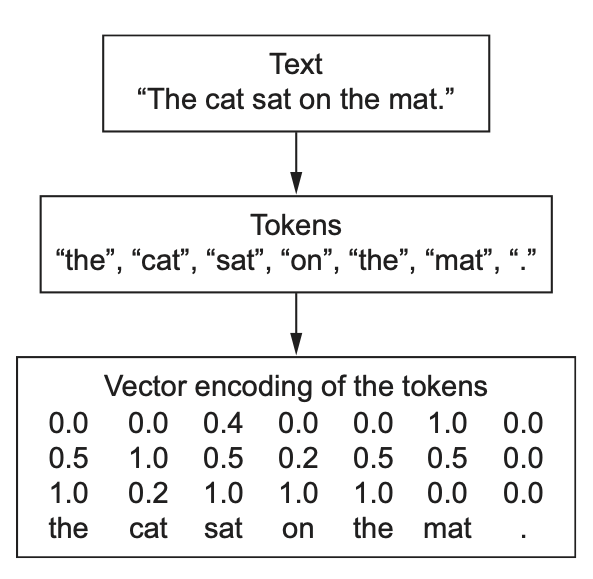
\includegraphics[width=0.4\textwidth]{fig/DLR_6_1_WE.png}
\caption{Representing words as word emnbeddings (Chollet and Allair, 2018, Fig. 6.1)}
\end{figure}

\end{frame}


\begin{frame}{Word embeddings vs. One-Hot}

\begin{figure}[h]
\centering
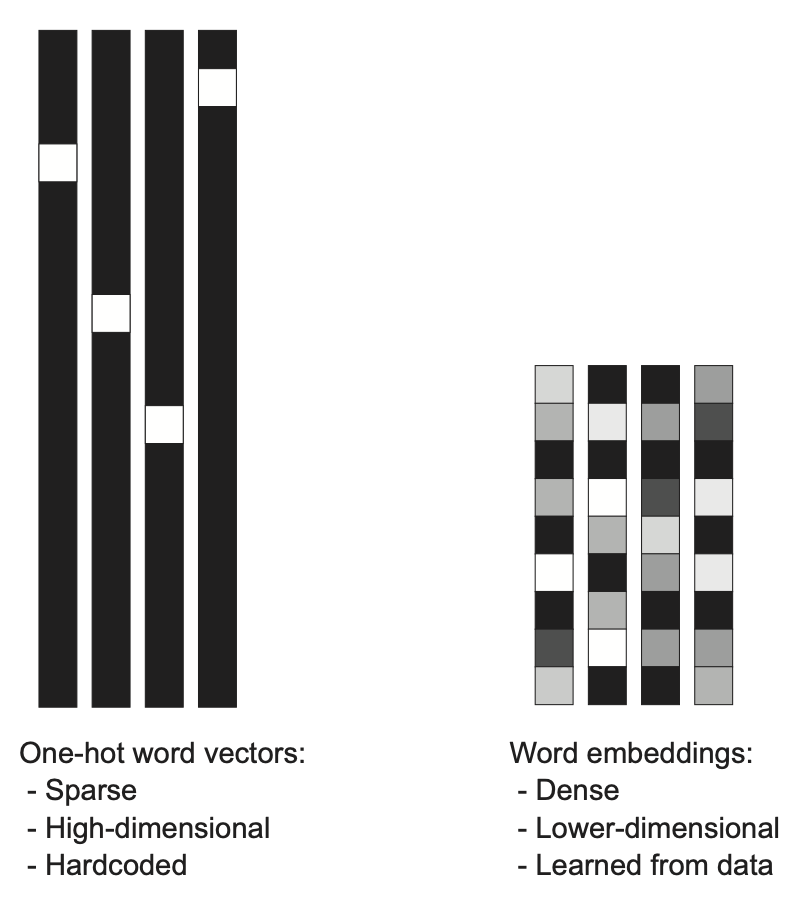
\includegraphics[width=0.5\textwidth]{fig/DLR_6_2_WE_VS_OH.png}
\caption{One-Hot vs. Word embeddings (Chollet and Allair, 2018, Fig. 6.2)}
\end{figure}

\end{frame}

\begin{frame}{Word embeddings}

\begin{itemize}
\item A word type represent {\color{uured} meaning in a low-dimensional semanitic space Word embeddings}
\item The distributional hypothesis:
\begin{itemize}
  \item Harris (1954) and Firth (1957): \\ ``A word is characterized by the company it keeps''
  \item Semantics (broadly defined) is captured by  {\color{uured} context}
\end{itemize}
\item Lots of different embeddings: \\ \texttt{word2vec}, GloVe, Probabilistic Embeddings
\end{itemize}

\begin{figure}[h]
\centering
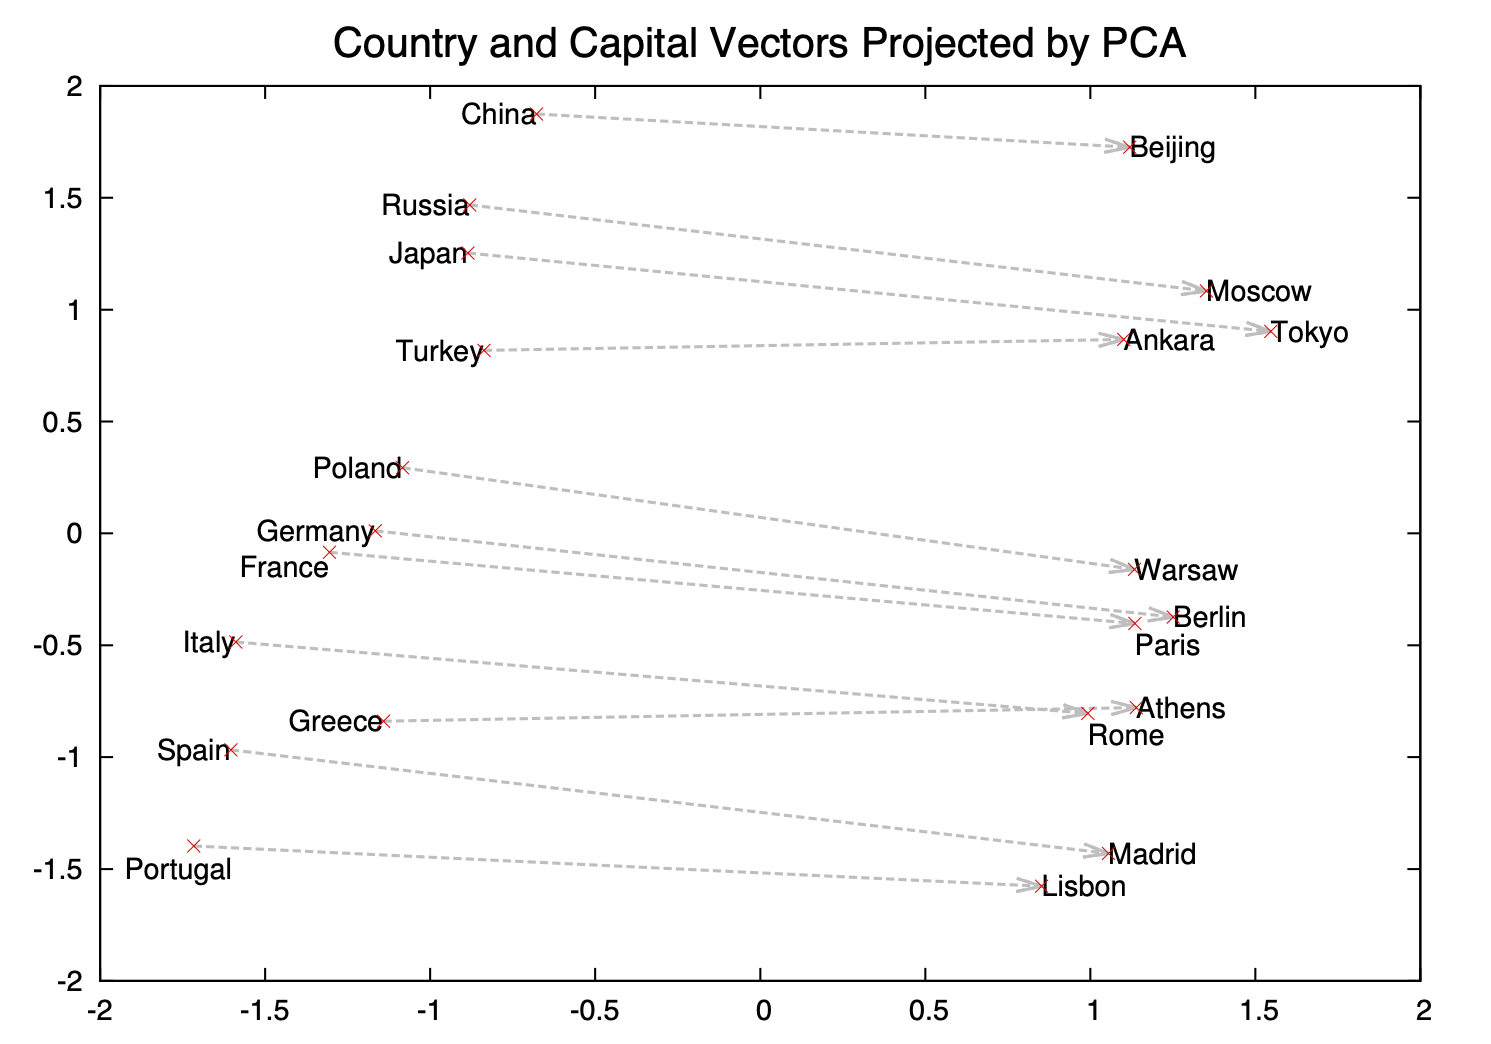
\includegraphics[width=0.6\textwidth]{fig/Mikolov_2013_word_projections.png}
\caption{Word embedding properties (Mikolov et al, 2013)}
\end{figure}

\end{frame}


\begin{frame}{Context Matters!}

\begin{figure}[h]
\centering
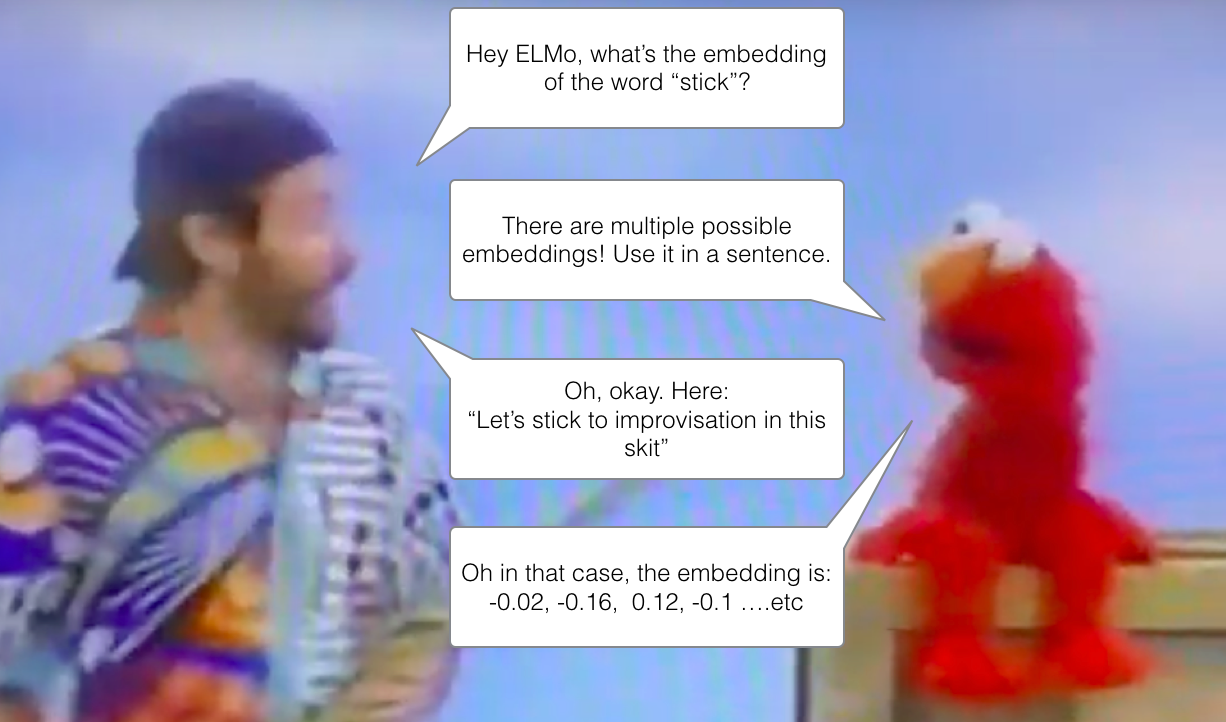
\includegraphics[width=0.9\textwidth]{fig/elmo-embedding-robin-williams.png}
\caption{Context matters (Alammar, 2020)}
\end{figure}

\end{frame}


\section{Recurrent Neural Networks}

\begin{frame}{Recurrent Neural Networks}

\begin{itemize}
\item Recurrent Neural Networks, Recurrent Nets, RNN, ...
\item Modeling of {\color{uured} temporal data structures}, such as
\begin{itemize}
\item Time series data
\item Sequences of words (language models)
\end{itemize}
\pause
\item Examples of applications:
\begin{itemize}
\item Text classification
\item Sequence / word classification
\item Time series predictions
\end{itemize}

\end{itemize}

\end{frame}

\begin{frame}{Recurrent Neural Networks}

\begin{figure}[h]
\centering
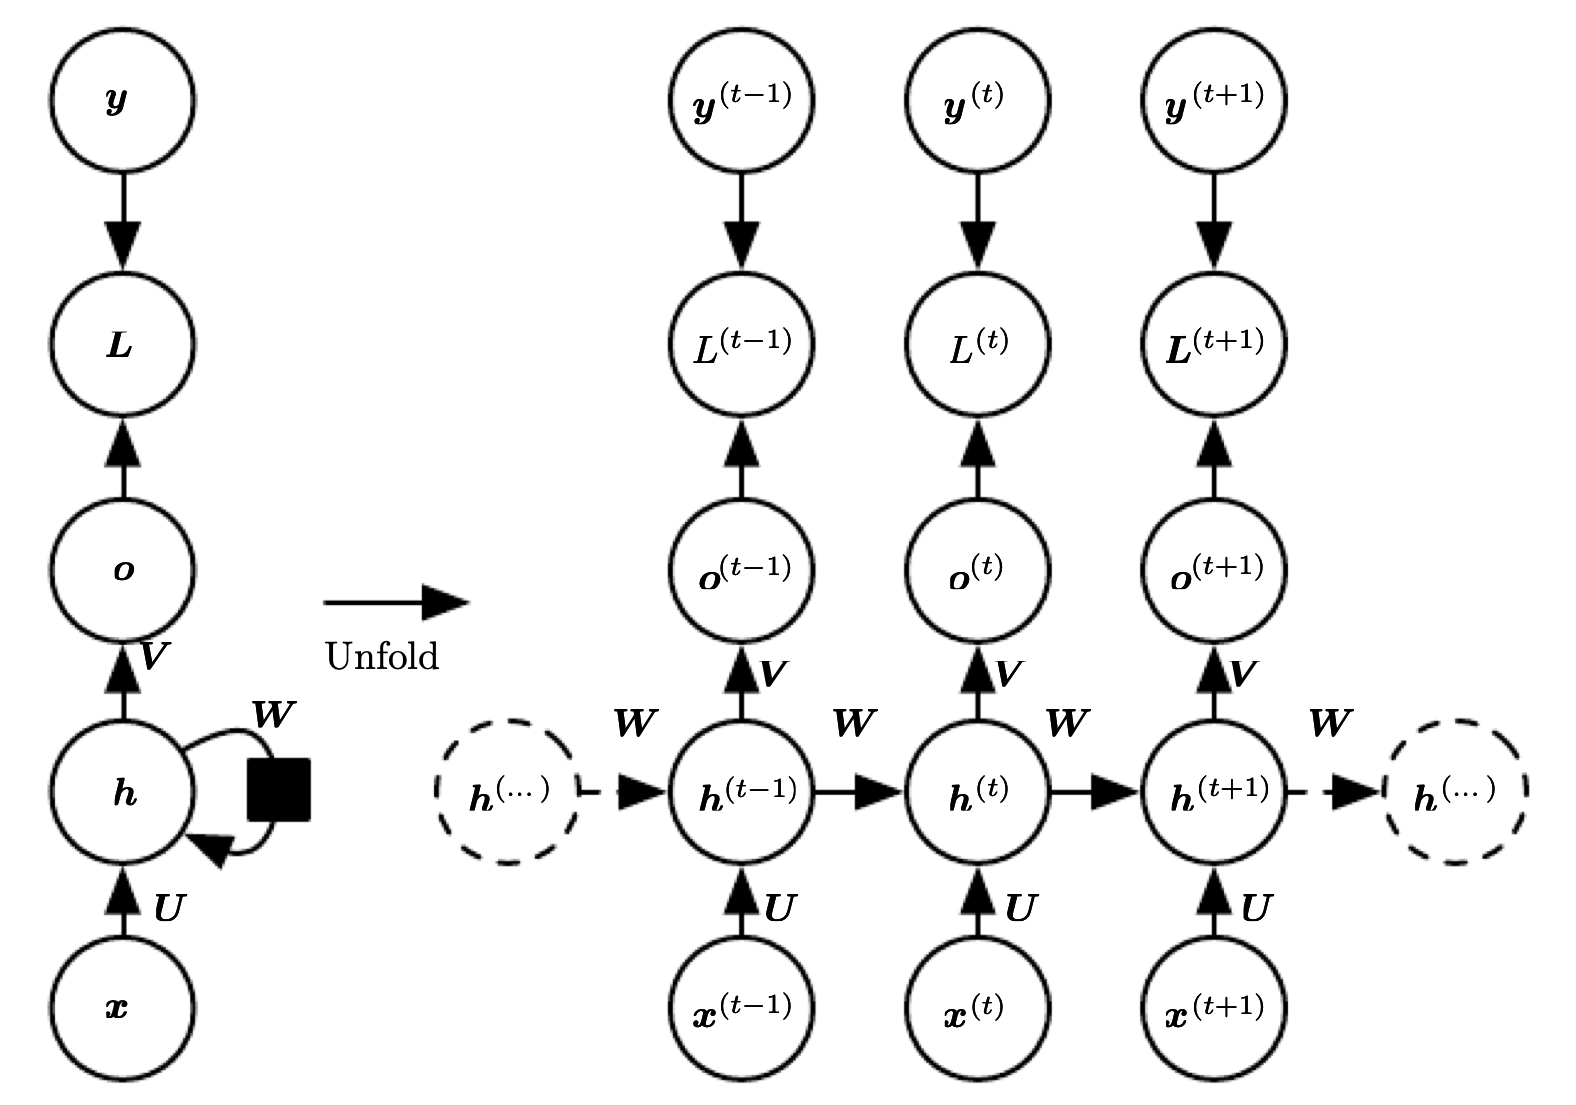
\includegraphics[width=0.9\textwidth]{fig/DL_10_3_RNN.png}
\caption{Recurrent Neural Network (Goodfellow et al, 2017, Fig. 10.3)}
\end{figure}

\end{frame}


\begin{frame}{Recurrent Neural Networks}

\begin{align*}
a_t &= b_t + W h_{t-1} + U x_t \\
h_t &= \sigma{a_t} \\
o_t &= c + V h_{t} \\
\hat{y}_t &= \text{softmax}(o_t)
\end{align*}

Think of $h_t$ as the "state" at timepoint $t$

\end{frame}



\begin{frame}{Recurrent network with one output}

\begin{figure}[h]
\centering
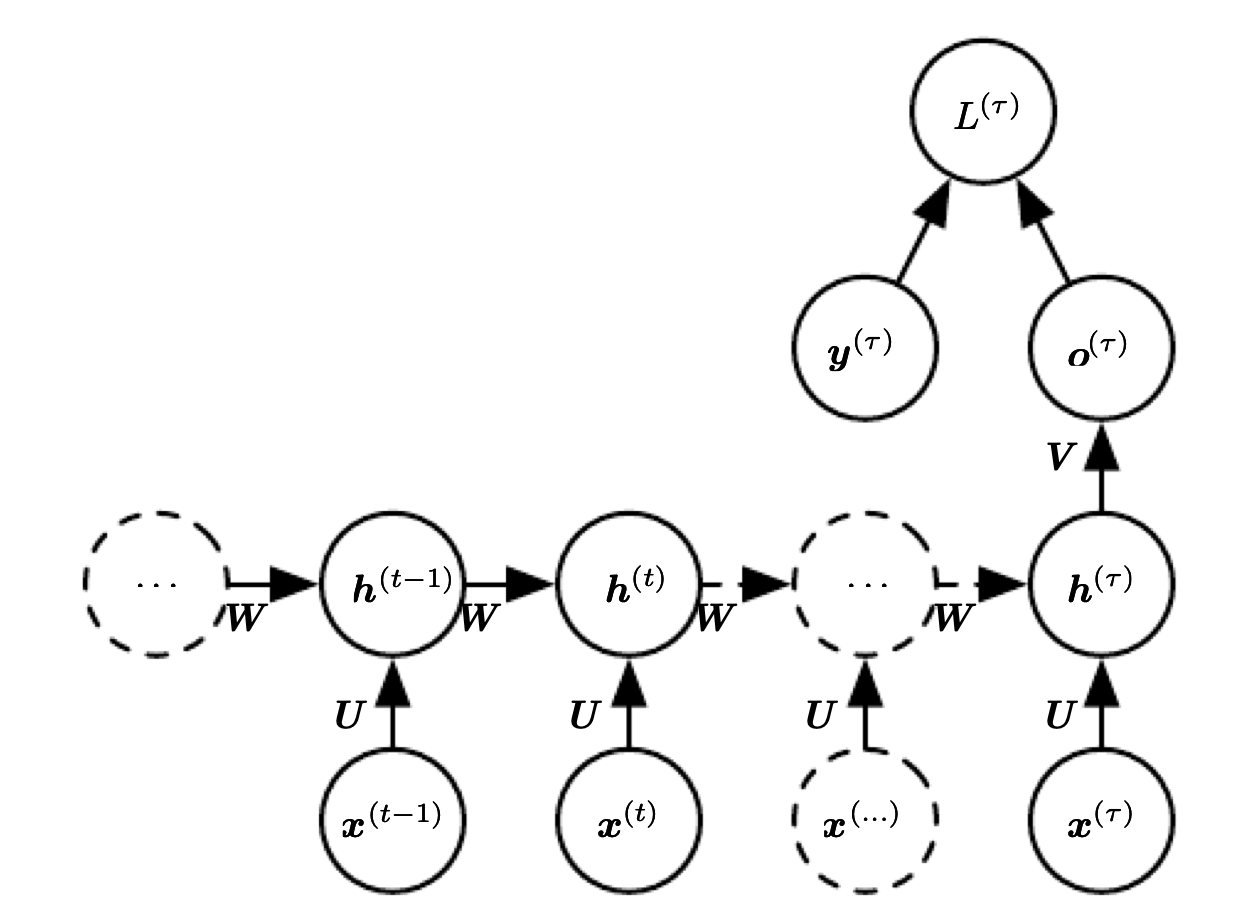
\includegraphics[width=0.9\textwidth]{fig/DL_10_5_RNN_one_class.png}
\caption{Recurrent Neural Network with one output (Goodfellow et al, 2017, Fig. 10.5)}
\end{figure}

\end{frame}

\begin{frame}{Sequence to Sequence: Encoder-Decoder}

\begin{figure}[h]
\centering
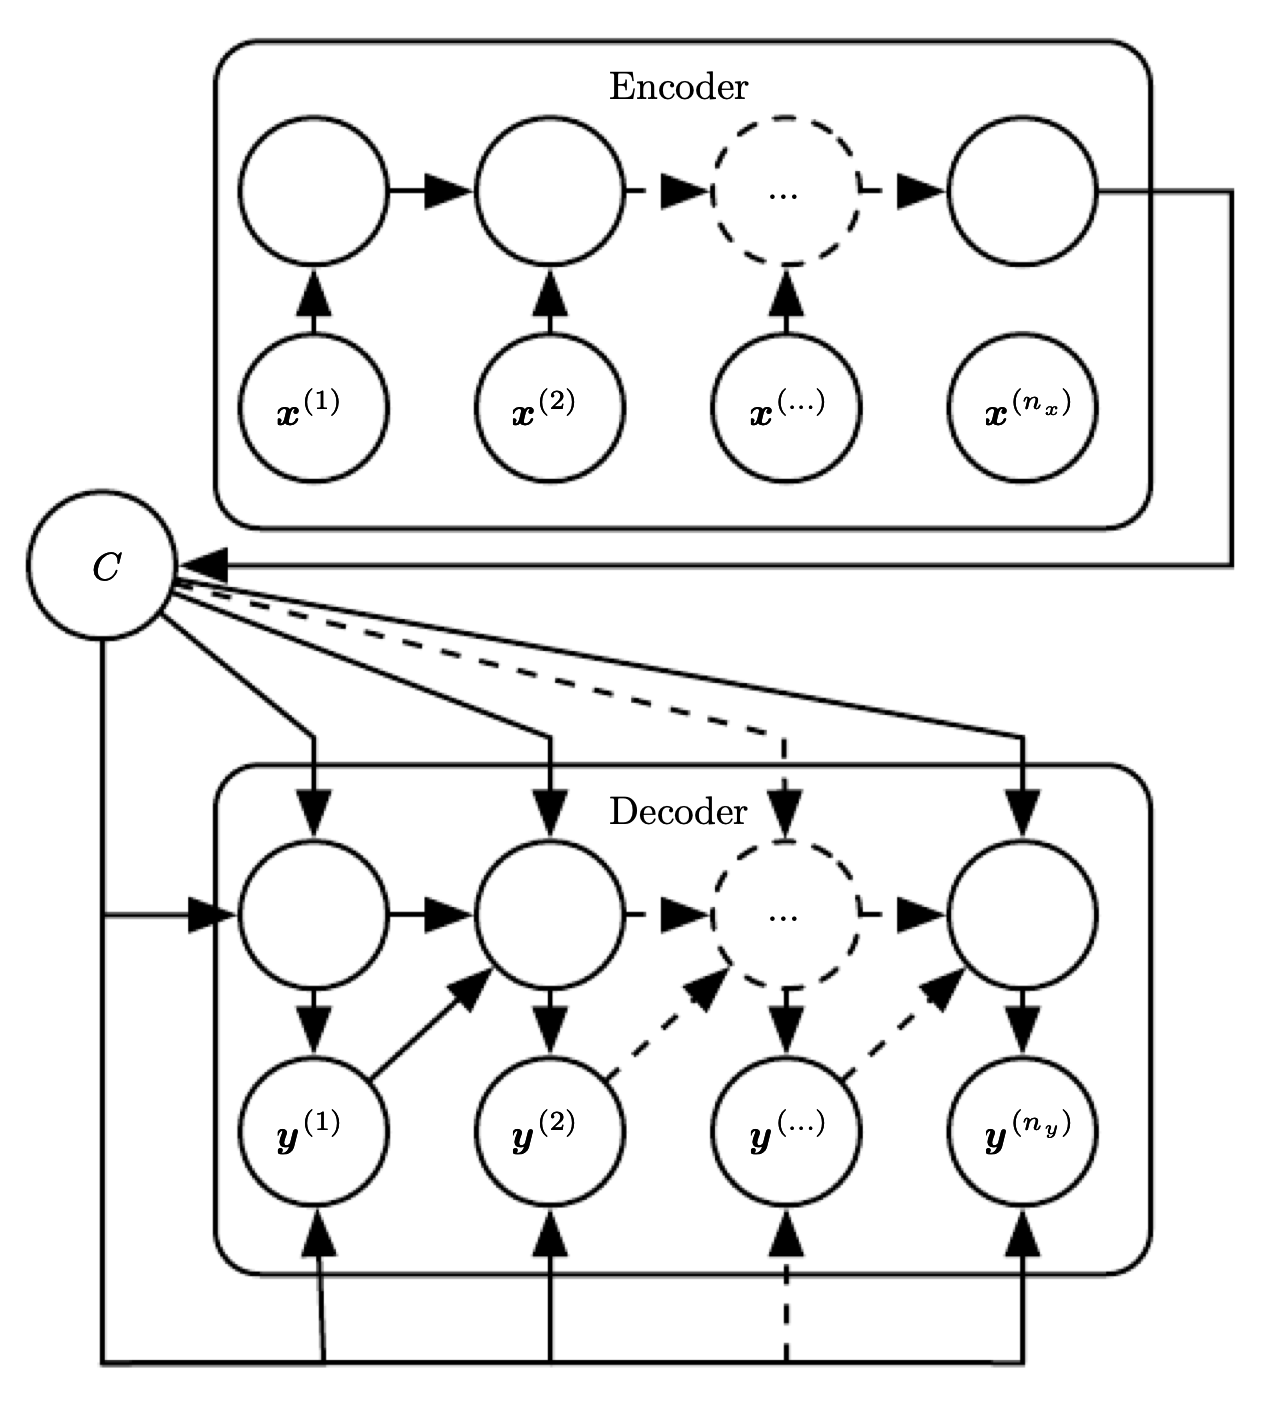
\includegraphics[width=0.7\textwidth]{fig/DL_10_12_Encoder_Decoder.png}
\caption{Encoder-Decoder Recurrent Networks (Goodfellow et al, 2017, Fig. 10.12)}
\end{figure}

\end{frame}


\begin{frame}{Problems with RNN}

\begin{itemize}
\item Predicting sequences of {\color{uured} different lengths}
\item {\color{uured} Exploding and vanishing} gradients
\item {\color{uured} Long-term}  dependencies
\end{itemize}
% TODO: Add 10.36-10.39 on the vanishing and exploding gradient

\end{frame}

\begin{frame}{Bi-Directional RNN}

\begin{figure}[h]
\centering
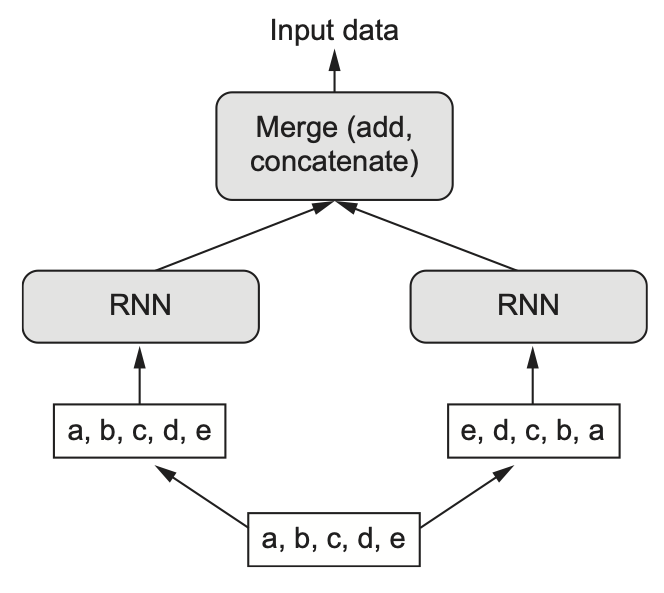
\includegraphics[width=0.8\textwidth]{fig/DLR_6_21_BiRNN}
\caption{Bi-Directional RNN (Chollet and Allaire, 2018, Fig. 6.21)}
\end{figure}

\end{frame}



\subsection{LSTM}


\begin{frame}{Long Short-Term Memory (LSTM)}

\begin{figure}[h]
\centering
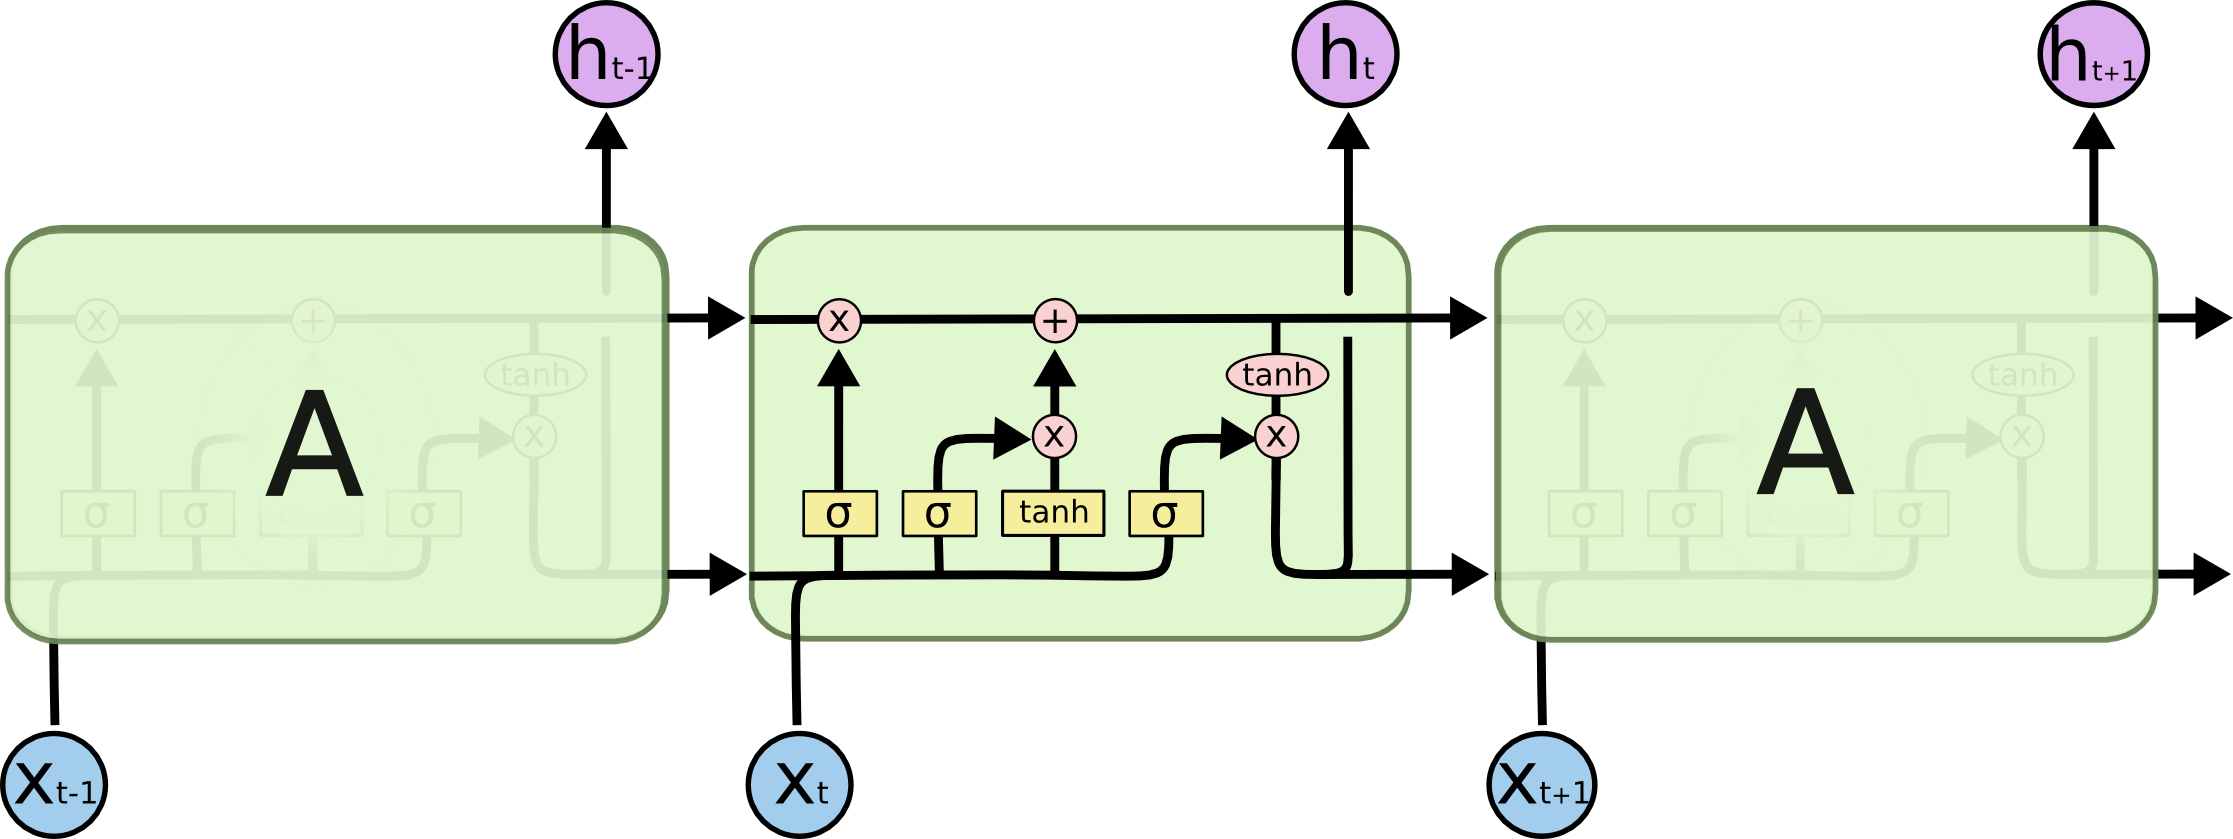
\includegraphics[width=1\textwidth]{fig/Olah_LSTM1.png}
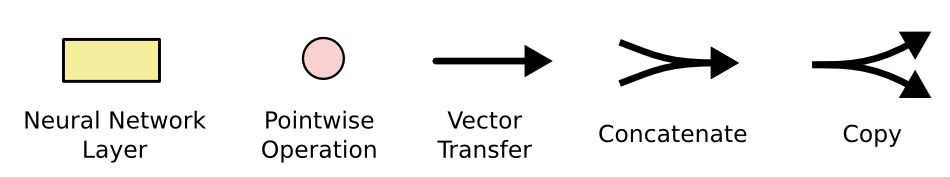
\includegraphics[width=1\textwidth]{fig/Olah_LSTM1b.png}
\caption{The LSTM (Olah, 2015)}
\end{figure}

\end{frame}


\begin{frame}{LSTM cell state}

\begin{figure}[h]
\centering
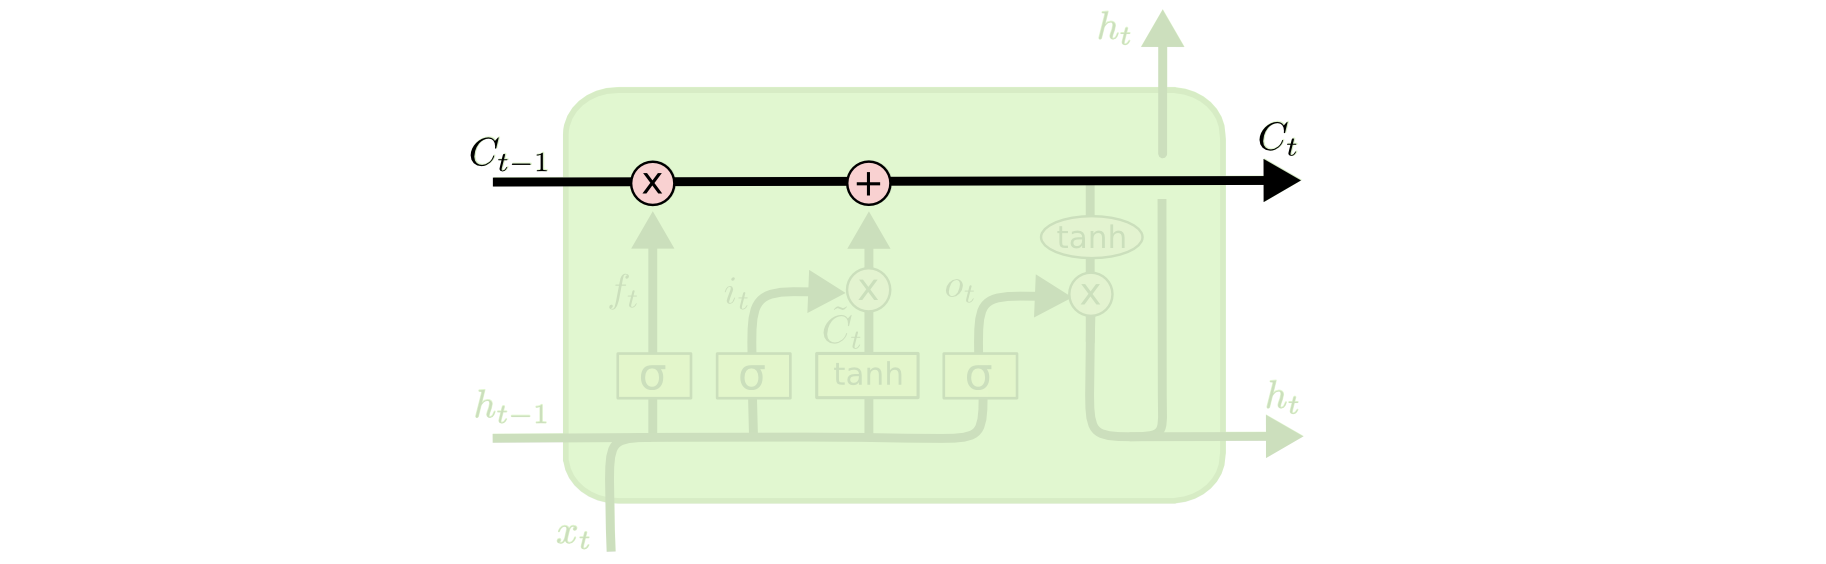
\includegraphics[width=1\textwidth]{fig/Olah_LSTM2.png}
\caption{LSTM cell state, i.e. "carrybelt" (Olah, 2015)}
\end{figure}

\end{frame}

\begin{frame}{LSTM forget gate}

\begin{figure}[h]
\centering
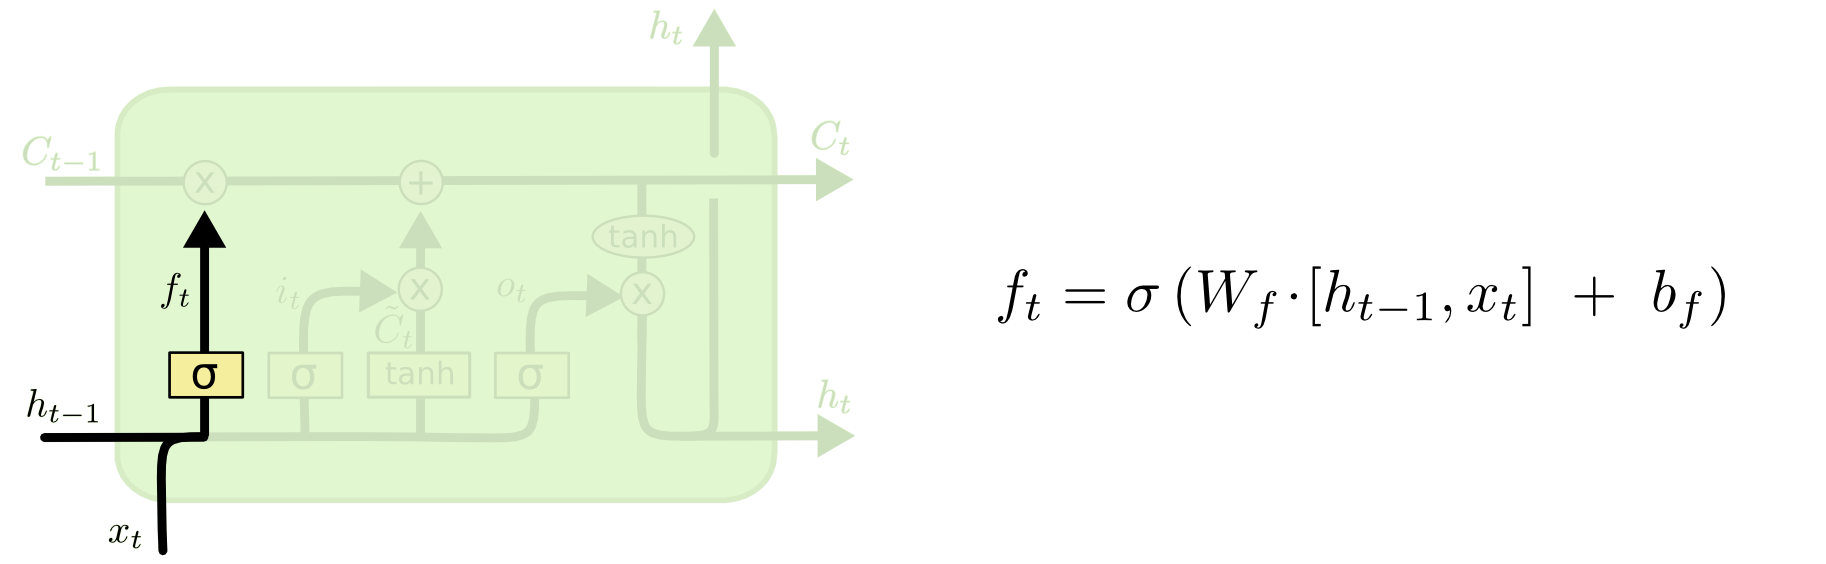
\includegraphics[width=1\textwidth]{fig/Olah_LSTM3_forget.png}
\caption{LSTM forget gate (Olah, 2015)}
\end{figure}

\end{frame}

\begin{frame}{LSTM input gate}

\begin{figure}[h]
\centering
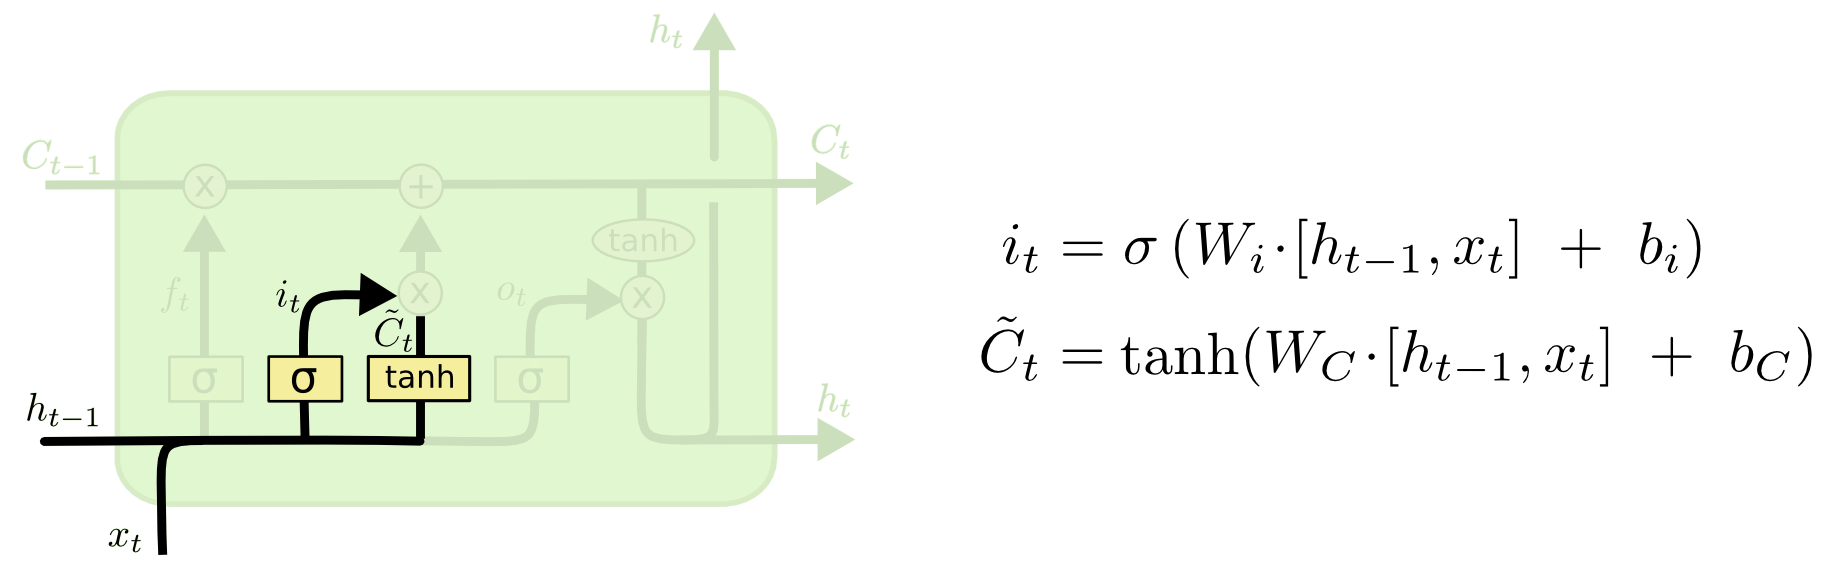
\includegraphics[width=1\textwidth]{fig/Olah_LSTM3_update.png}
\caption{LSTM input gate (Olah, 2015)}
\end{figure}

\end{frame}

\begin{frame}{LSTM cell state update}

\begin{figure}[h]
\centering
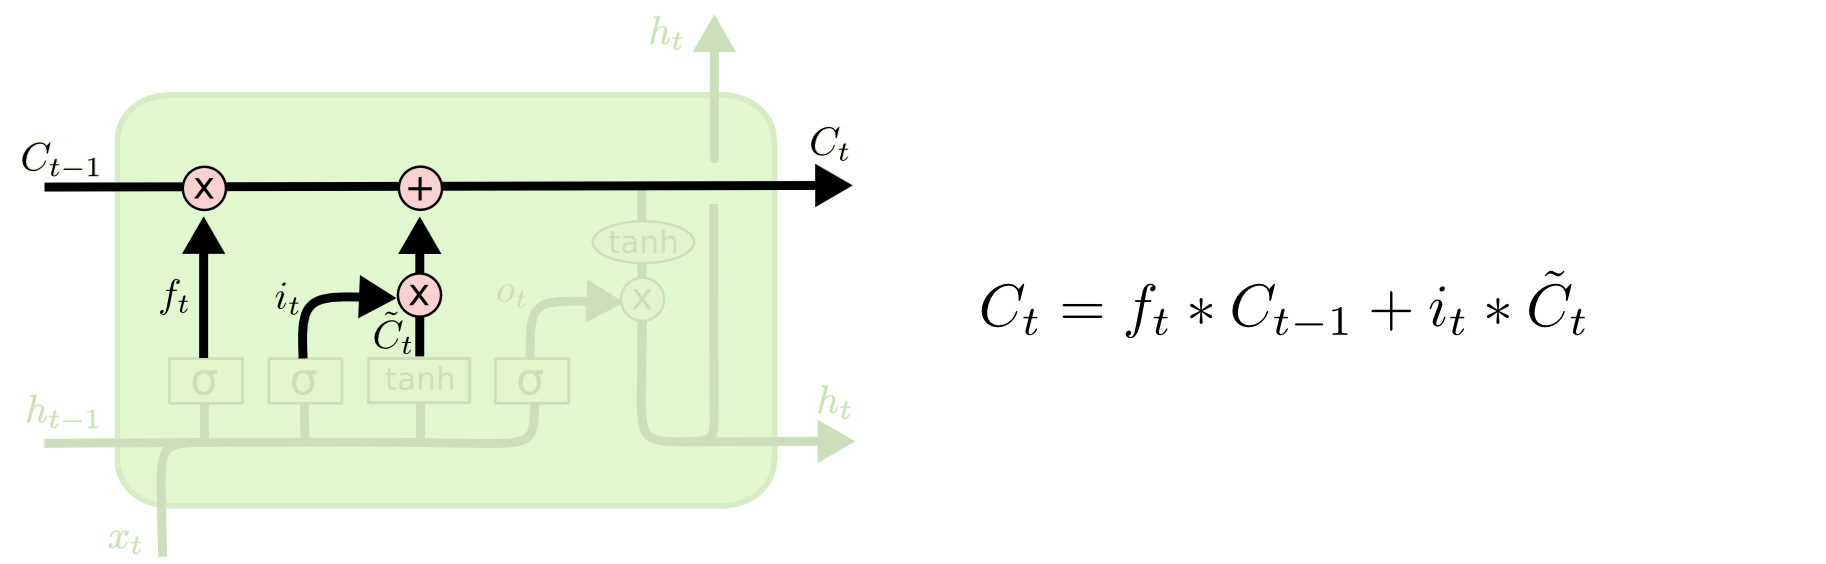
\includegraphics[width=1\textwidth]{fig/Olah_LSTM3_update2.png}
\caption{Update cell state (Olah, 2015)}
\end{figure}

\end{frame}

\begin{frame}{LSTM output gate}

\begin{figure}[h]
\centering
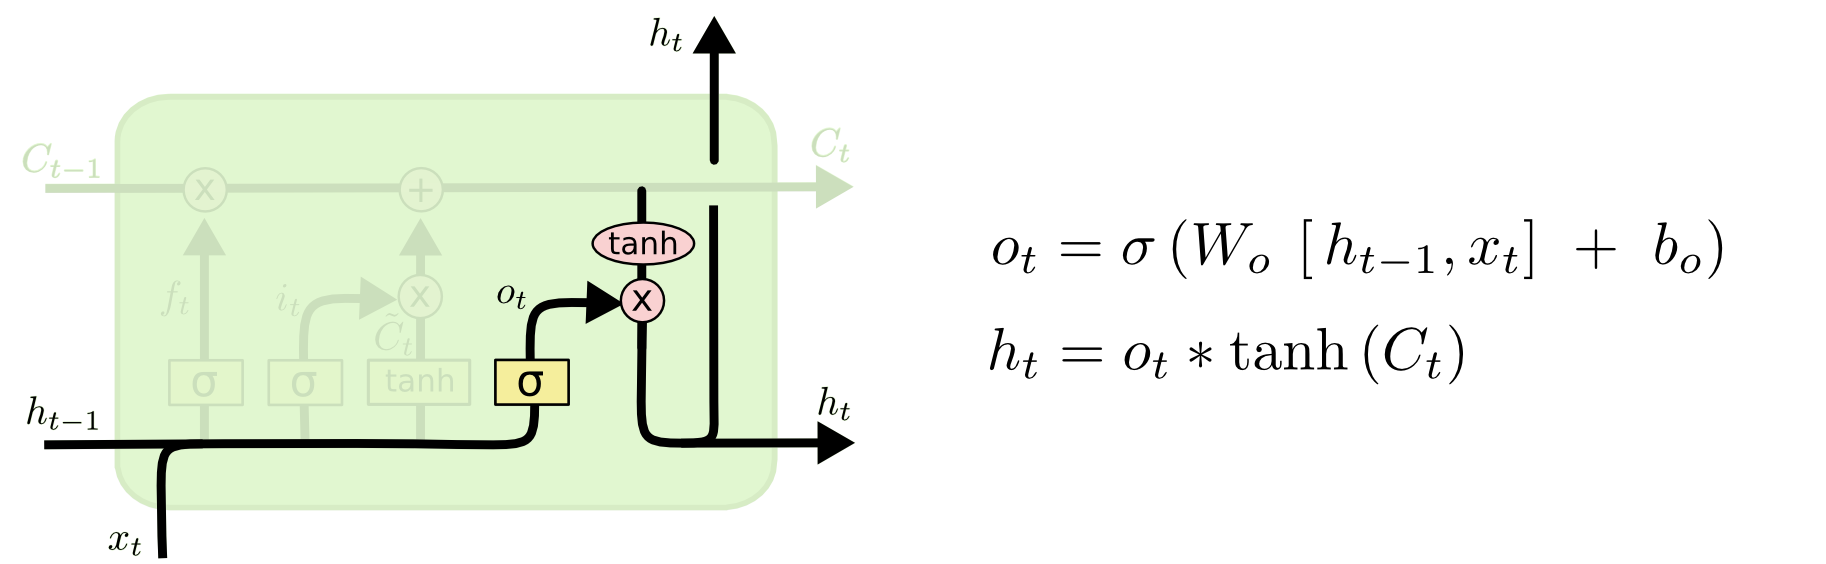
\includegraphics[width=1\textwidth]{fig/Olah_LSTM3_output.png}
\caption{LSTM output gate (Olah, 2015)}
\end{figure}

\end{frame}


\begin{frame}{Problems}

\begin{itemize}
\item Still a {\color{uured} recurrent structure},\\(vanishing and exploding gradients)
\item Long-term dependencies still difficult
\item Hard to do {\color{uured} transfer learning}
\end{itemize}


\end{frame}


\section{Attention and Transformers}

\begin{frame}{Transformer}

\begin{itemize}
\item Introduced in 2017 in Vaswani et al. (2017)
\item Behind the recent progress in NLP: BERT, GPT-2, GPT-3, etc.
\pause
\item Becoming de-facto standard in industry and academia
\pause
\item Brings {\color{uured} transfer learning} to NLP
\pause
\item Two large benefits:
\begin{itemize}
\item Enables more {\color{uured} parallelism}
\item Better handling of {\color{uured} long-range dependencies}
%\item Enables {\color{uured} deeper} networks
\end{itemize}
\end{itemize}

\end{frame}



\begin{frame}{A Sequence-to-Sequence Model}

\begin{figure}[h]
\centering
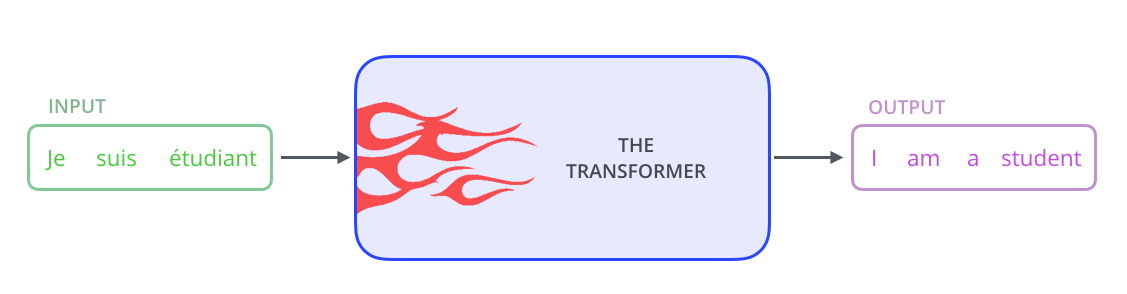
\includegraphics[width=1\textwidth]{fig/alammar_the_transformer_3.png}
\caption{Attention (Vaswani et al., 2017)}
\end{figure}

\end{frame}


\begin{frame}{Stacked Encoder-Decoder Structure}

\begin{figure}[h]
\centering
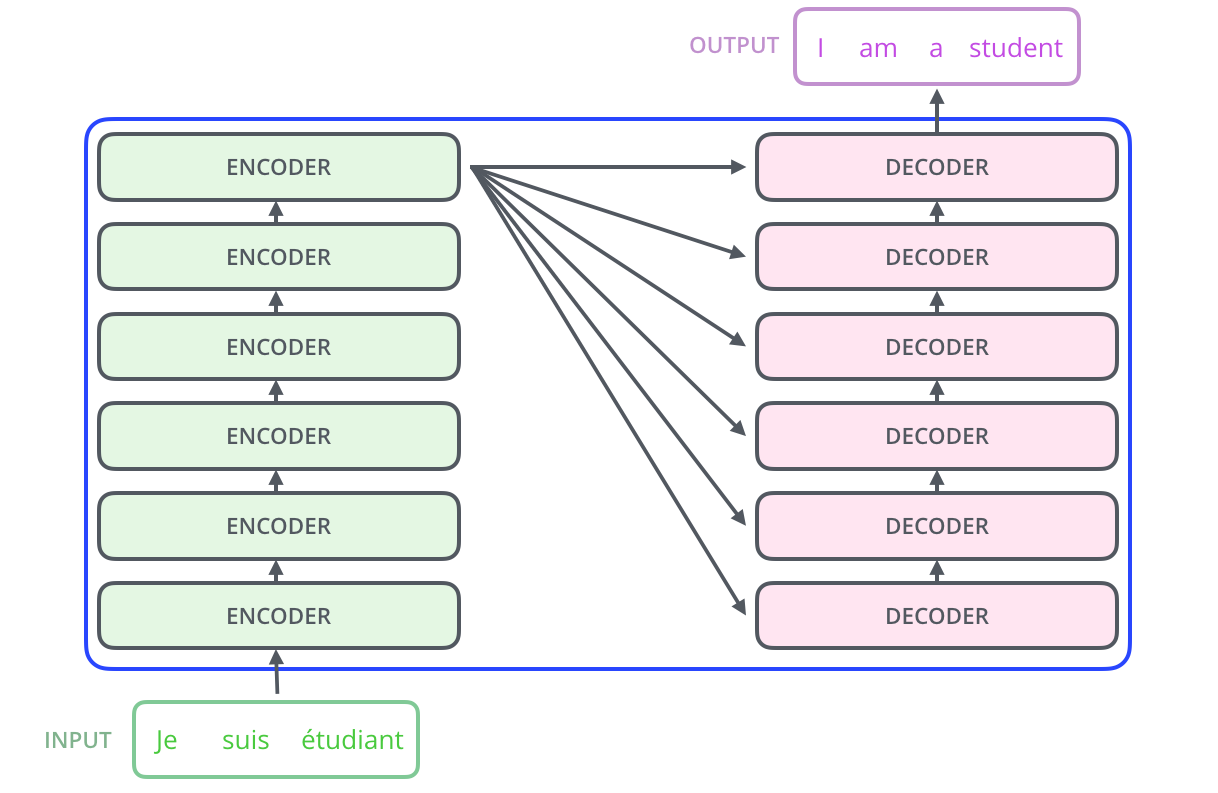
\includegraphics[width=1\textwidth]{fig/alammar_The_transformer_encoder_decoder_stack}
\caption{Attention (Vaswani et al., 2017)}
\end{figure}

\end{frame}


\begin{frame}{Transformer}

\begin{figure}[h]
\centering
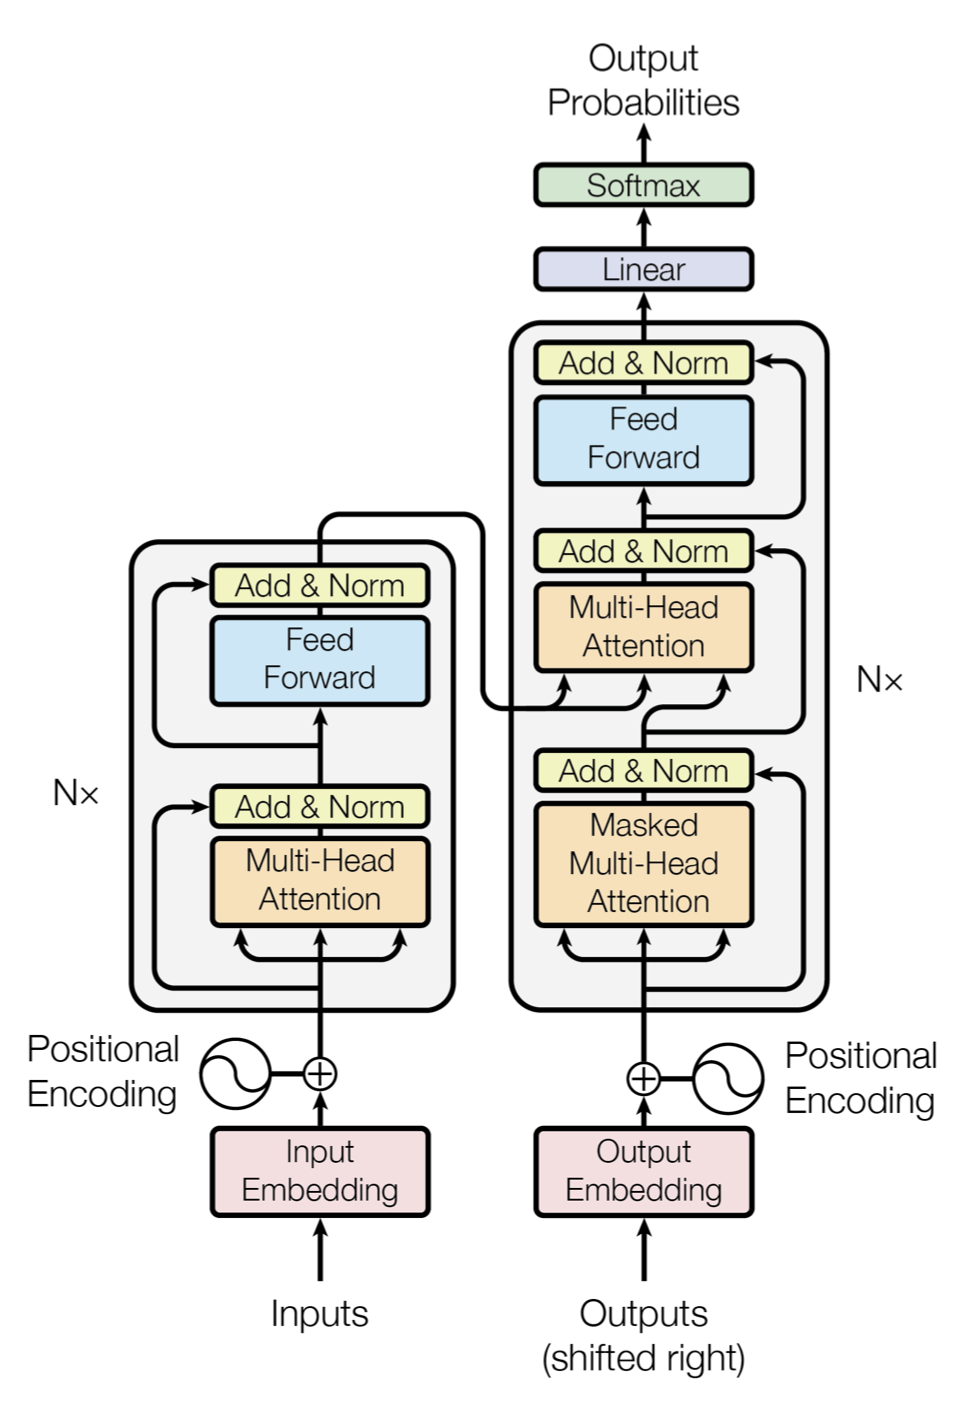
\includegraphics[width=0.5\textwidth]{fig/Vaswani_1_transformer.png}
\caption{The Transformer Architecture (Vaswani et al., 2017)}
\end{figure}



\end{frame}

\begin{frame}{The encoder vs. the decoder}

\begin{itemize}
\item Encoder:
\begin{itemize}
\item Input: words (embeddings)
\item Output: contextualized embeddings
\end{itemize}
\item Decoder:
\begin{itemize}
\item Input: contextualized embeddings {\color{uured} and previous words} (embeddings)
\item Output: words (embeddings)
\end{itemize}
\end{itemize}
\end{frame}



\begin{frame}{The Encoder Layer}

\begin{figure}[h]
\centering
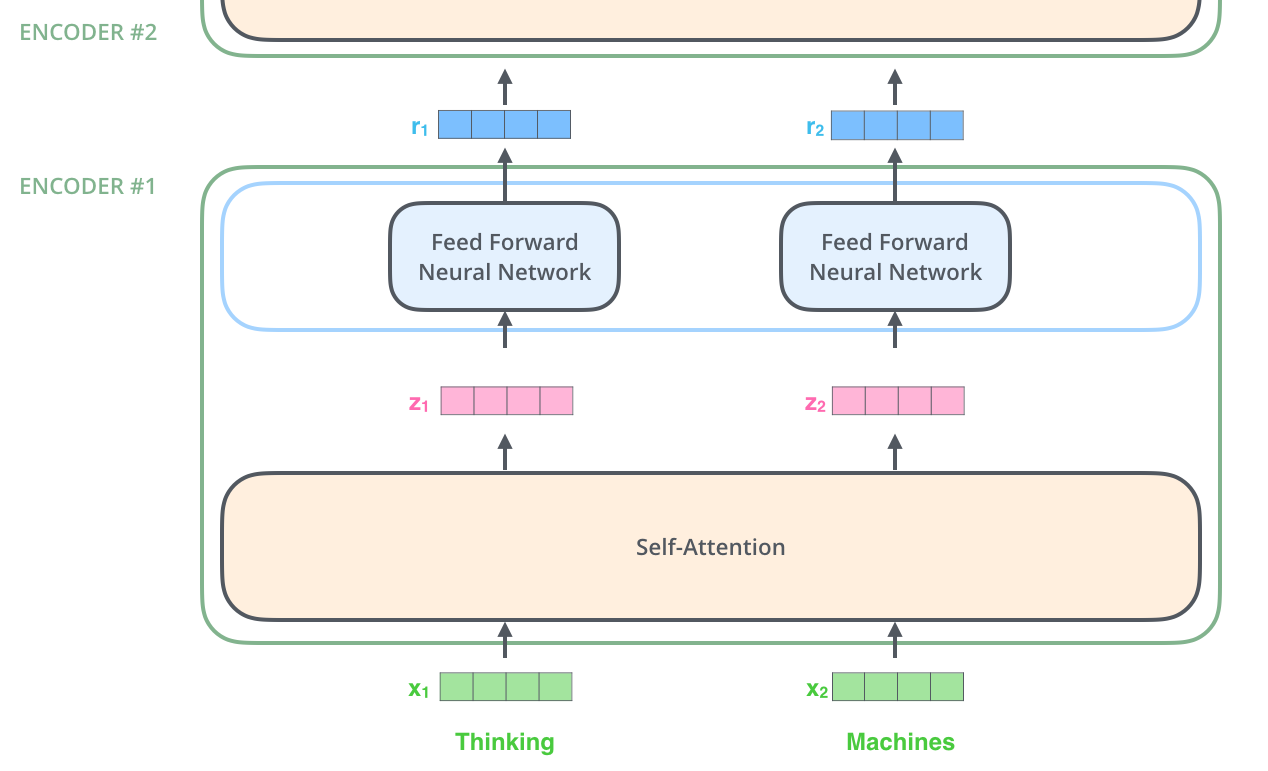
\includegraphics[width=1\textwidth]{fig/alammar_encoder_with_tensors_2.png}
\caption{The Encoder Layer (Alammar, 2018)}
\end{figure}

\end{frame}


\subsection{Attention}

\begin{frame}{Scaled Dot-Product Attention}

\begin{figure}[h]
\centering
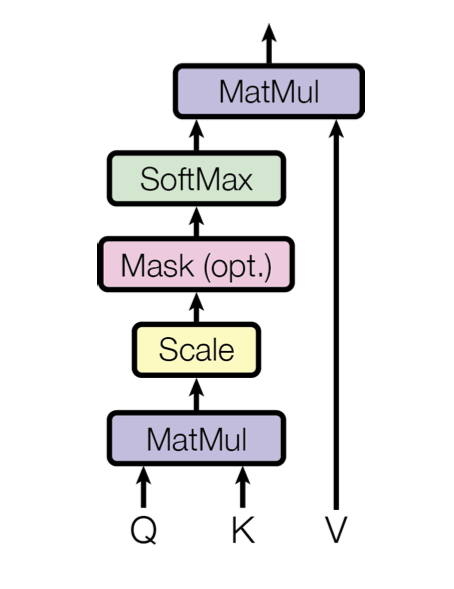
\includegraphics[width=0.4\textwidth]{fig/Vaswani_2_scaled_dot.png}
\caption{Scaled Dot-Product Attention (Vaswani et al., 2017)}
\end{figure}

\end{frame}


\begin{frame}{The encoder vs. the decoder}

\begin{itemize}
\item (Q)uery: Word $i$ query other words
\item (K)ey: The other words return their key to $i$
\item (V)alue: The value of the other words to $i$
\end{itemize}
\end{frame}


\begin{frame}{Computing Q, V and K}

\begin{figure}[h]
\centering
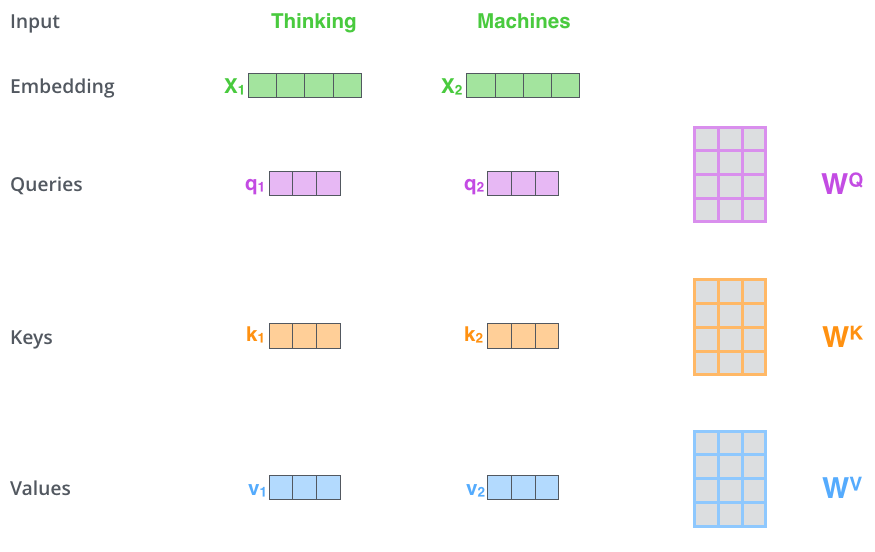
\includegraphics[width=1\textwidth]{fig/alammar_transformer_self_attention_vectors.png}
\caption{Attention heads (Alammar, 2018)}
\end{figure}

\end{frame}

\begin{frame}{Computing Self-Attention}

\begin{figure}[h]
\centering
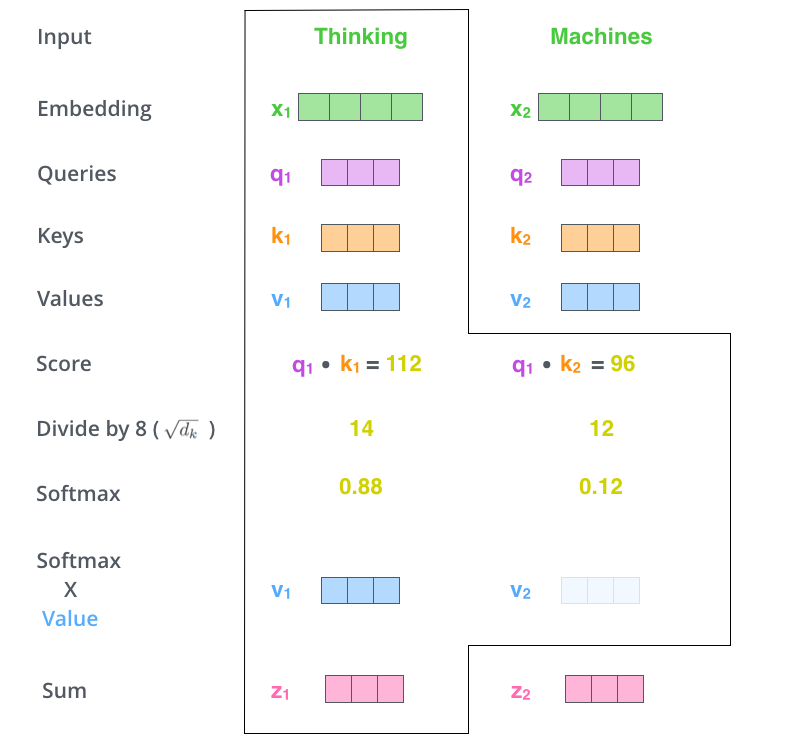
\includegraphics[width=0.8\textwidth]{fig/alammar_self-attention-output.png}
\caption{Attention (Alammar, 2018)}
\end{figure}

\end{frame}


\subsection{Multi-Head Attention}

\begin{frame}{Multi-Head Attention}

\begin{figure}[h]
\centering
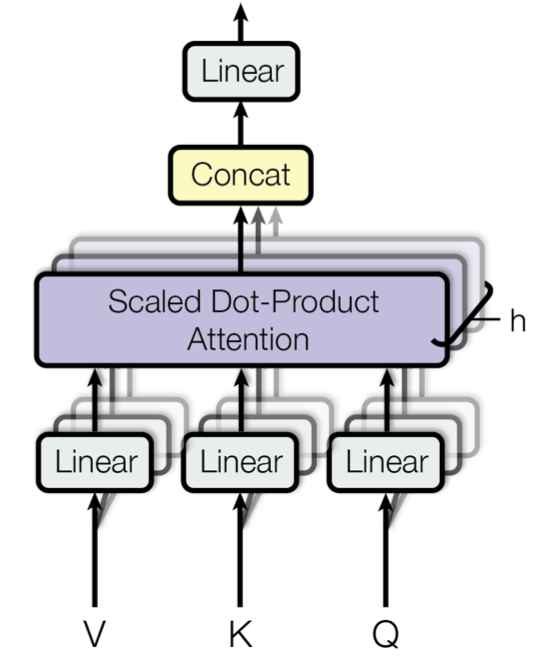
\includegraphics[width=0.4\textwidth]{fig/Vaswani_2_multi_head.png}
\caption{Scaled Dot-Product Attention (Vaswani et al., 2017)}
\end{figure}

\end{frame}


\begin{frame}{Attentions Heads}

\begin{figure}[h]
\centering
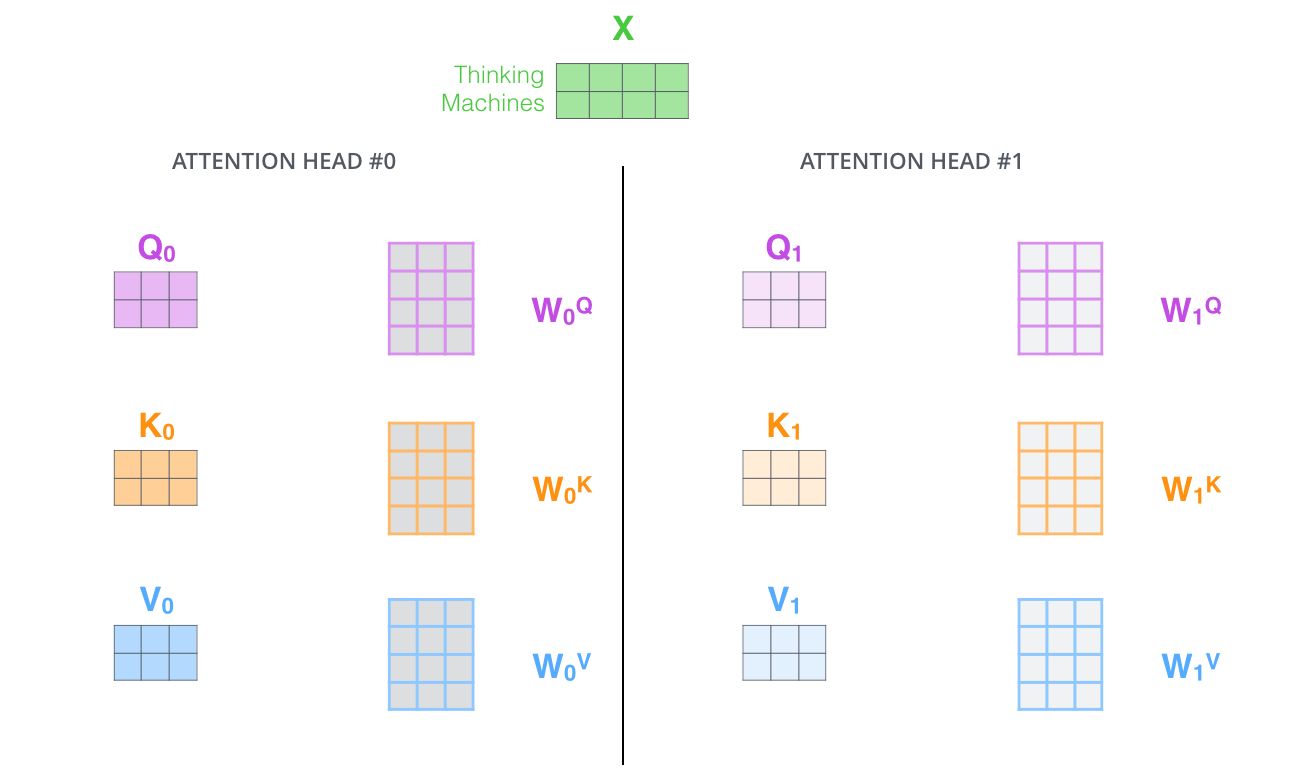
\includegraphics[width=1\textwidth]{fig/alammar_transformer_attention_heads_qkv.png}
\caption{Attention heads (Alammar, 2018)}
\end{figure}

\end{frame}


\begin{frame}{Multi-head attention}

\begin{figure}[h]
\centering
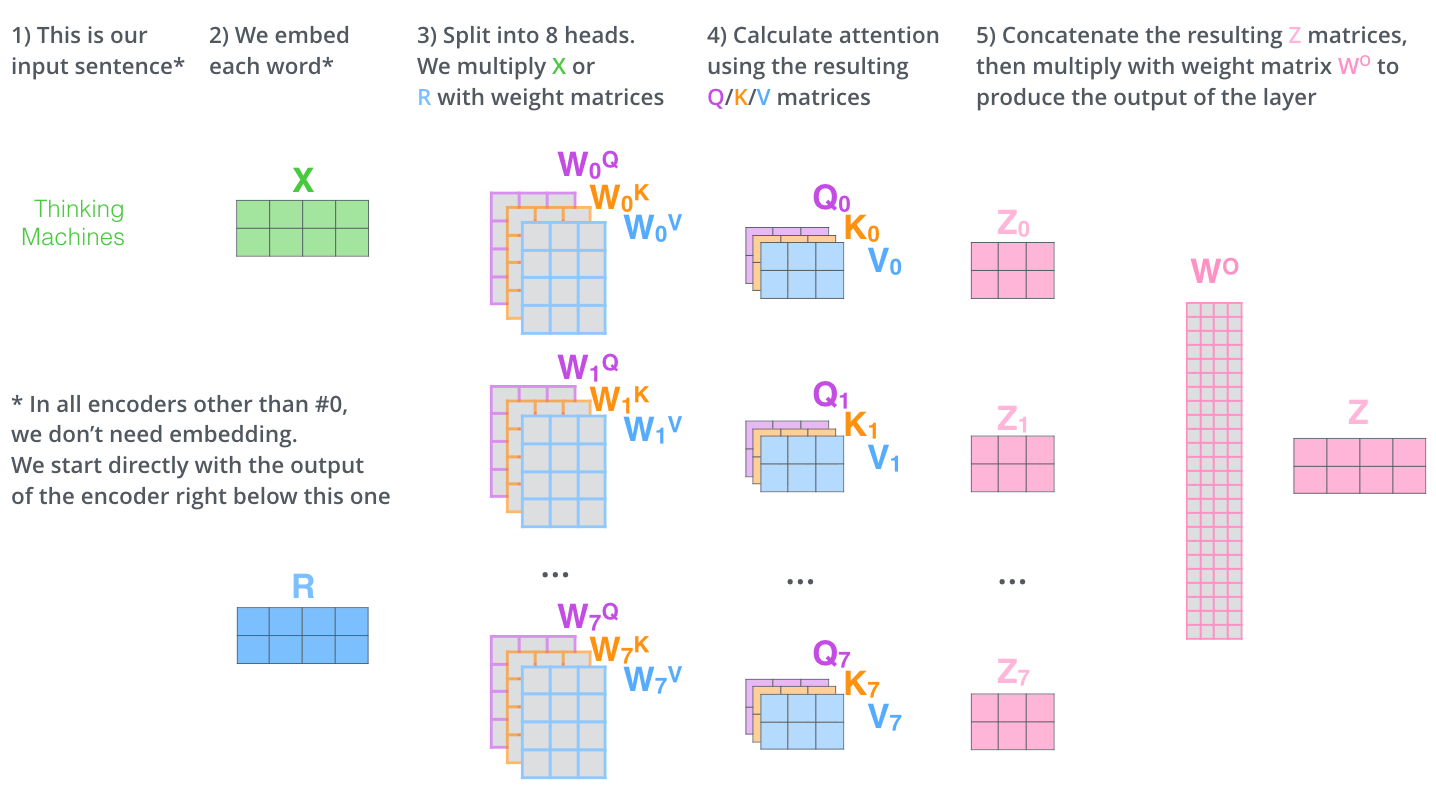
\includegraphics[width=1\textwidth]{fig/alammar_transformer_multi-headed_self-attention-recap.png}
\caption{Attention heads (Alammar, 2018)}
\end{figure}

\end{frame}


\begin{frame}{Multi-Head Attention example}

\begin{figure}[h]
\centering
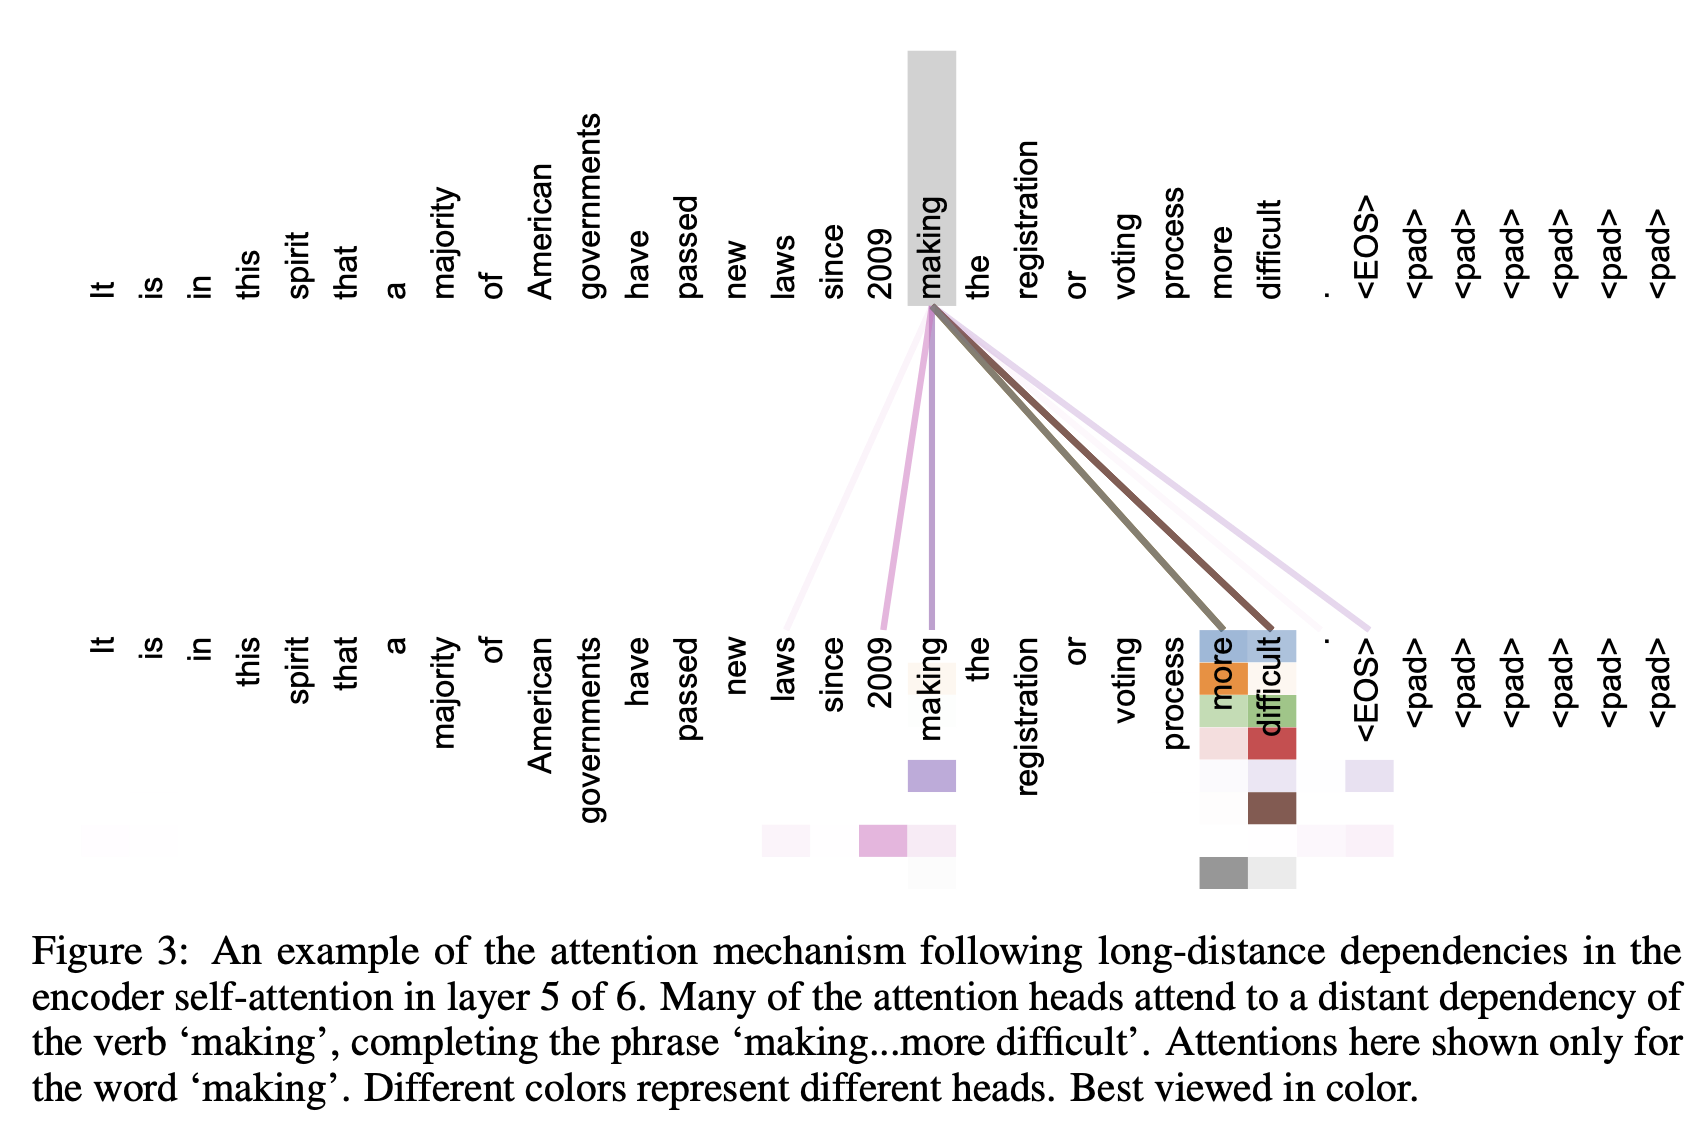
\includegraphics[width=1\textwidth]{fig/Vaswani_3_attention.png}
\caption{Attention (Vaswani et al., 2017)}
\end{figure}

\end{frame}

\subsection{Positional encoding}

\begin{frame}{Positional Encoding}

\begin{figure}[h]
\centering
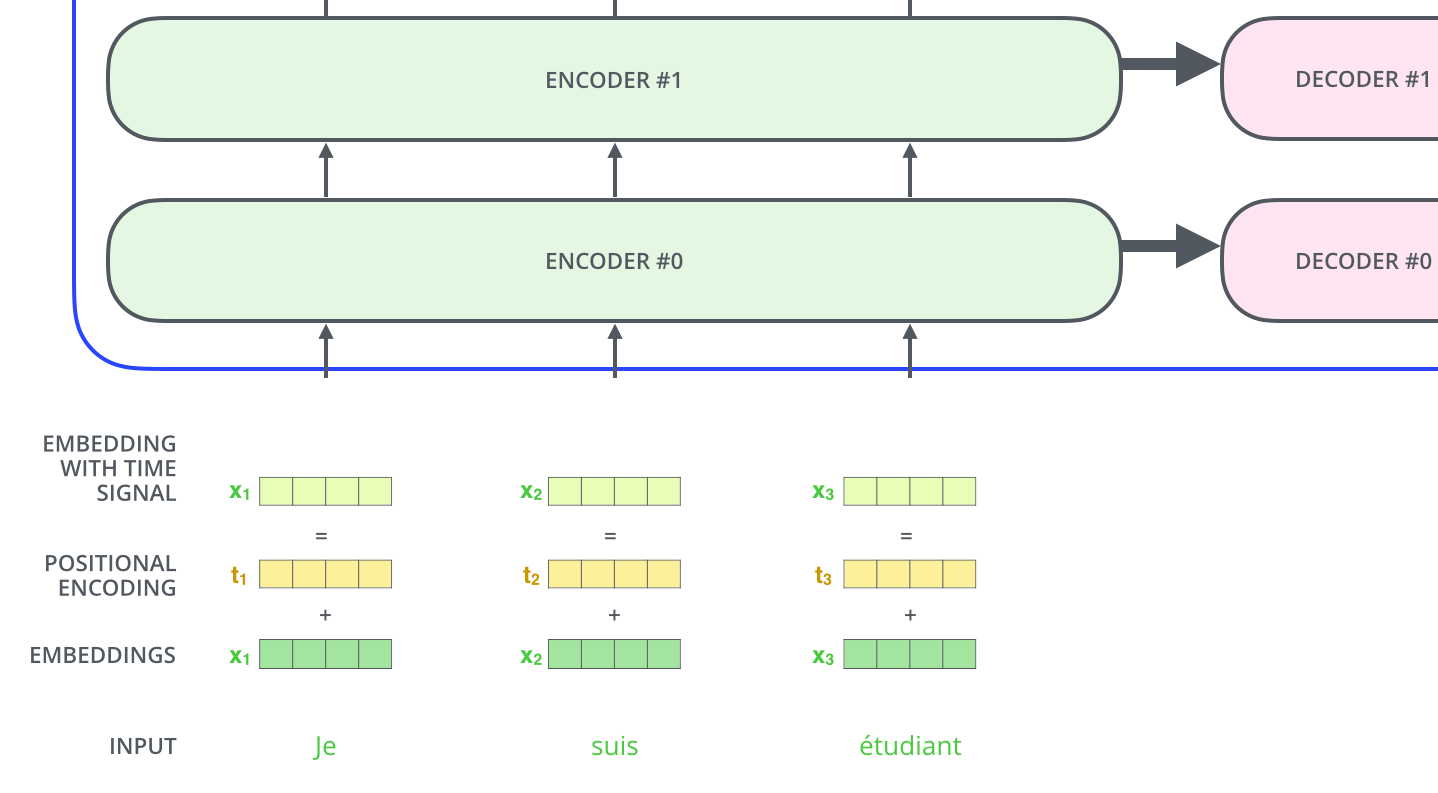
\includegraphics[width=1\textwidth]{fig/alammar_transformer_positional_encoding_vectors.png}
\caption{Attention heads (Alammar, 2018)}
\end{figure}

\end{frame}

\begin{frame}{Positional Encoding}

\begin{figure}[h]
\centering
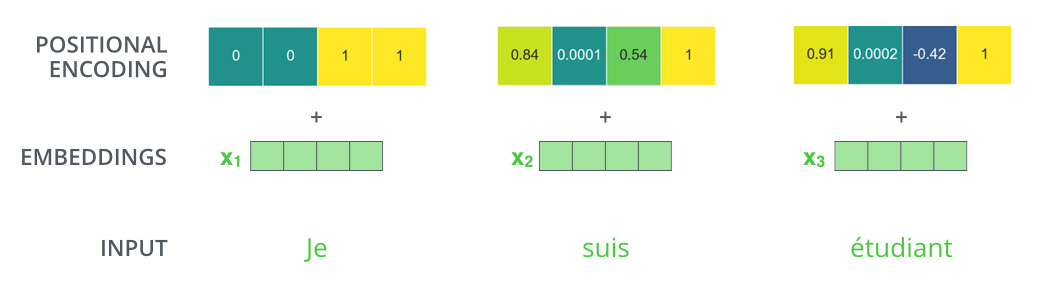
\includegraphics[width=1\textwidth]{fig/alammar_transformer_positional_encoding_example.png}
\caption{Adding positional encodings to embeddings (Alammar, 2018)}
\end{figure}

\end{frame}

\subsection{Add and Normalize}

\begin{frame}{Add and Normalize}

\begin{figure}[h]
\centering
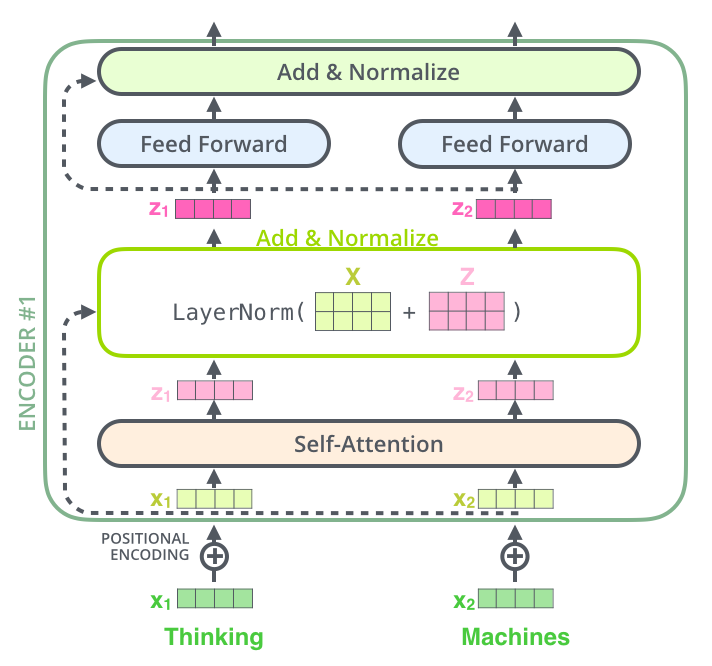
\includegraphics[width=0.8\textwidth]{fig/alammar_transformer_resideual_layer_norm_2.png}
\caption{Add and Normalize (Alammar, 2018)}
\end{figure}

\end{frame}



\begin{frame}{Transformer}

\begin{figure}[h]
\centering
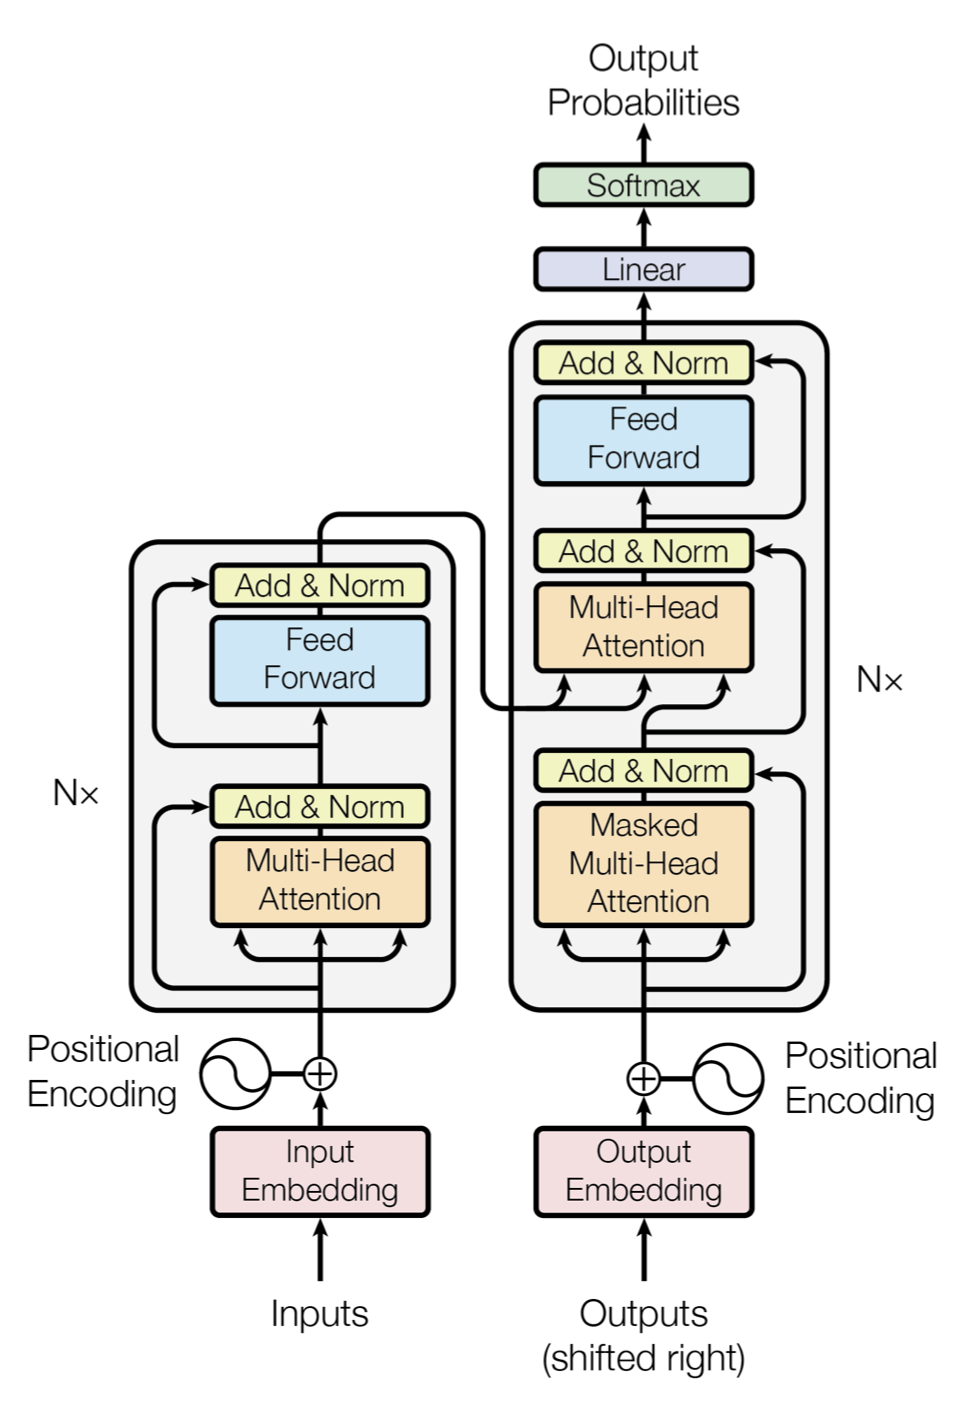
\includegraphics[width=0.5\textwidth]{fig/Vaswani_1_transformer.png}
\caption{The Transformer Architecture (Vaswani et al., 2017)}
\end{figure}

\end{frame}


%\begin{frame}{Transformer Decoder}
%\begin{figure}[h]
%\centering
%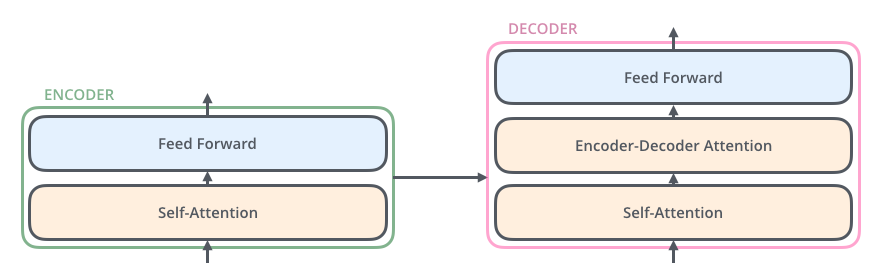
\includegraphics[width=1\textwidth]{fig/alammar_Transformer_decoder.png}
%\caption{Attention heads (Vaswani et al., 2017)}
%\end{figure}
%\end{frame}

\section{BERT}


\begin{frame}{BERT}

\begin{itemize}
\item Bidirectional Encoder Representations from Transformers
\item Introduced in 2018/2019 in Devlin et al. (2017)
\pause
\item {\color{uured} State-of-the-Art} in many text prediction tasks, such as
\begin{itemize}
\item Question-Answering
\item Named-Entity Recognition
\item Text Classification
\end{itemize}
\pause
\item Becoming the de facto new standard in industry and NLP
\pause
\item {\color{uured} Pre-trained} on a large number of books
\pause
\item Available both in English and Swedish (The National Library)
\end{itemize}

\end{frame}


\begin{frame}{BERT and transfer learning}

\begin{figure}[h]
\centering
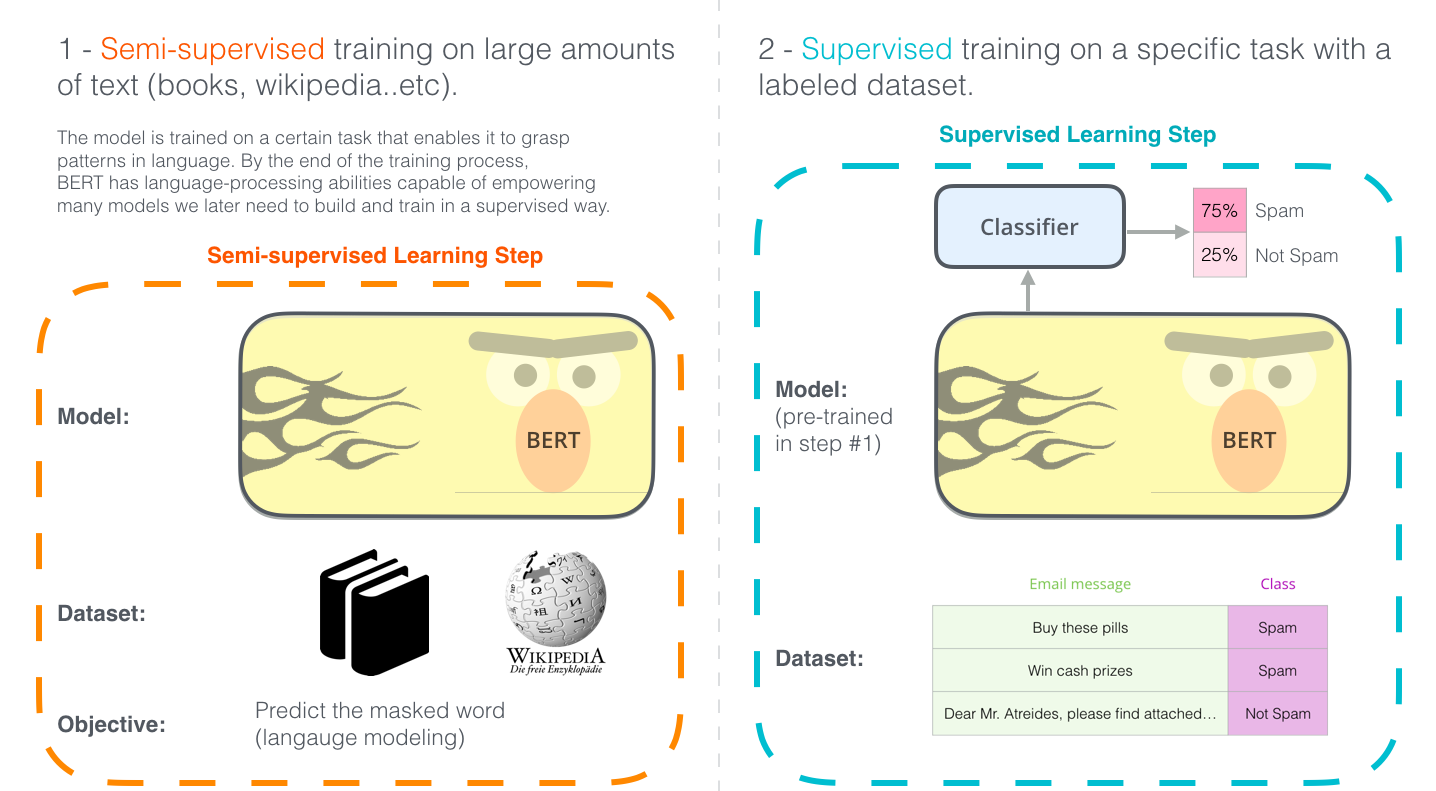
\includegraphics[width=1\textwidth]{fig/bert-transfer-learning.png}
\caption{Using BERT for Transfer Learning (Alammar, 2019)}
\end{figure}

\end{frame}


\begin{frame}{The BERT model}

\begin{figure}[h]
\centering
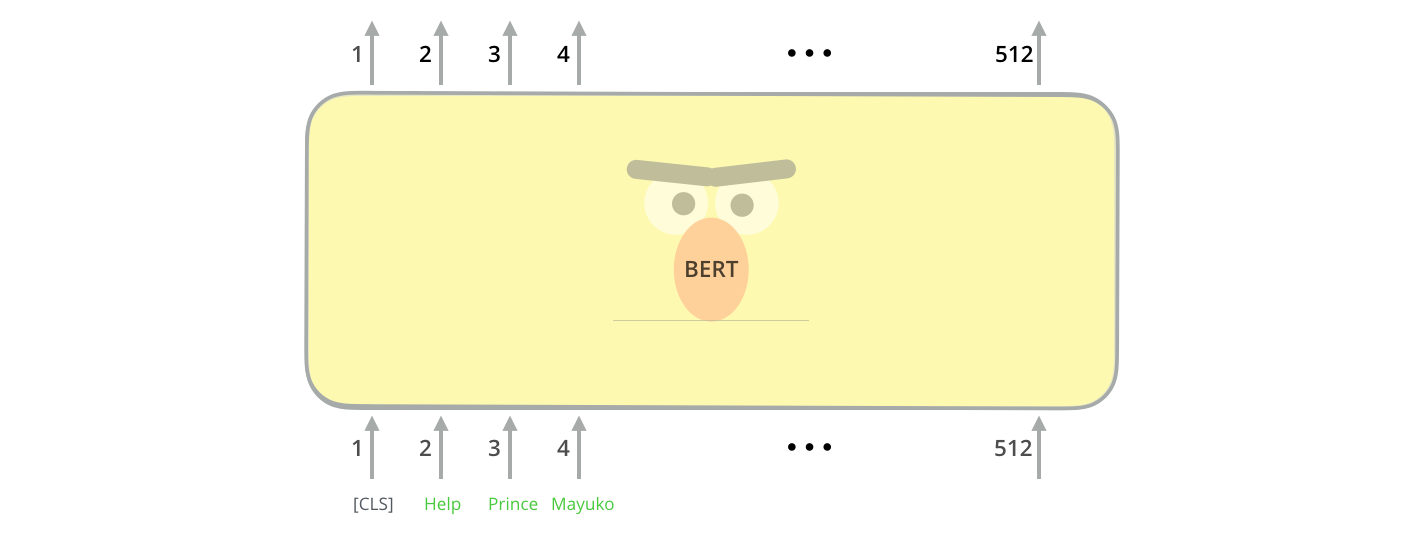
\includegraphics[width=0.9\textwidth]{fig/bert-input-output.png}
\caption{The BERT model (Alammar, 2019)}
\end{figure}

\end{frame}


\begin{frame}{BERT Architecture}

\begin{figure}[h]
\centering
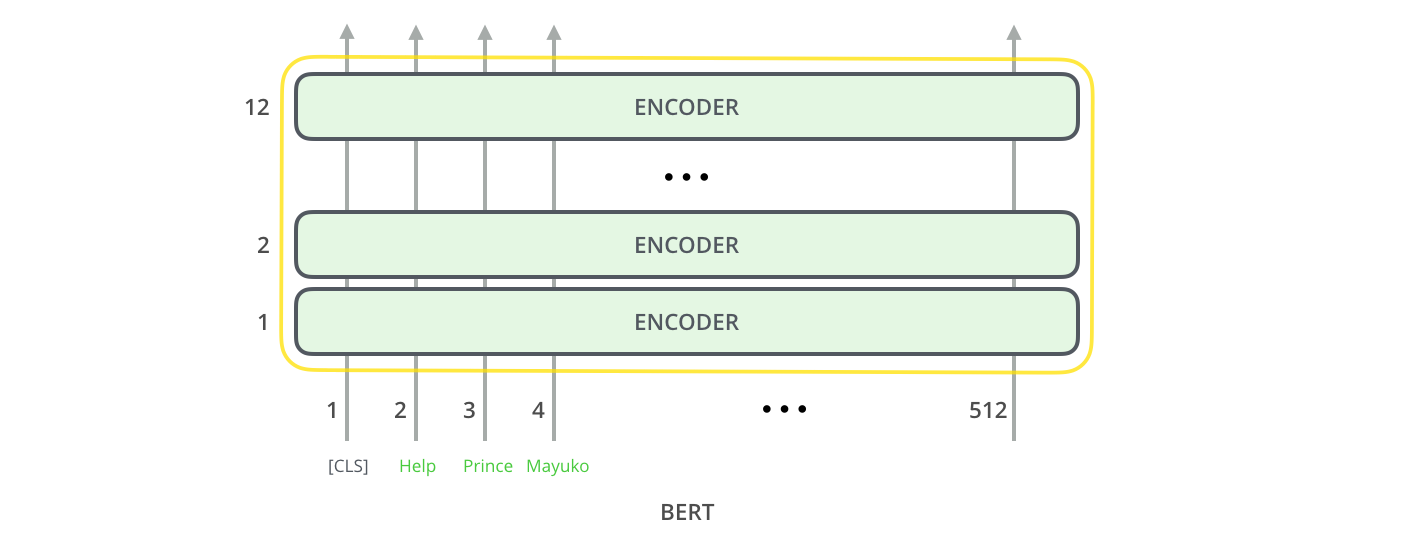
\includegraphics[width=0.9\textwidth]{fig/bert-encoders-input.png}
\caption{Opening up BERT (Vaswani et al., 2017)}
\end{figure}

\end{frame}



\subsection{Training BERT}


\begin{frame}{Task 1: Masked Language Model}

\begin{figure}[h]
\centering
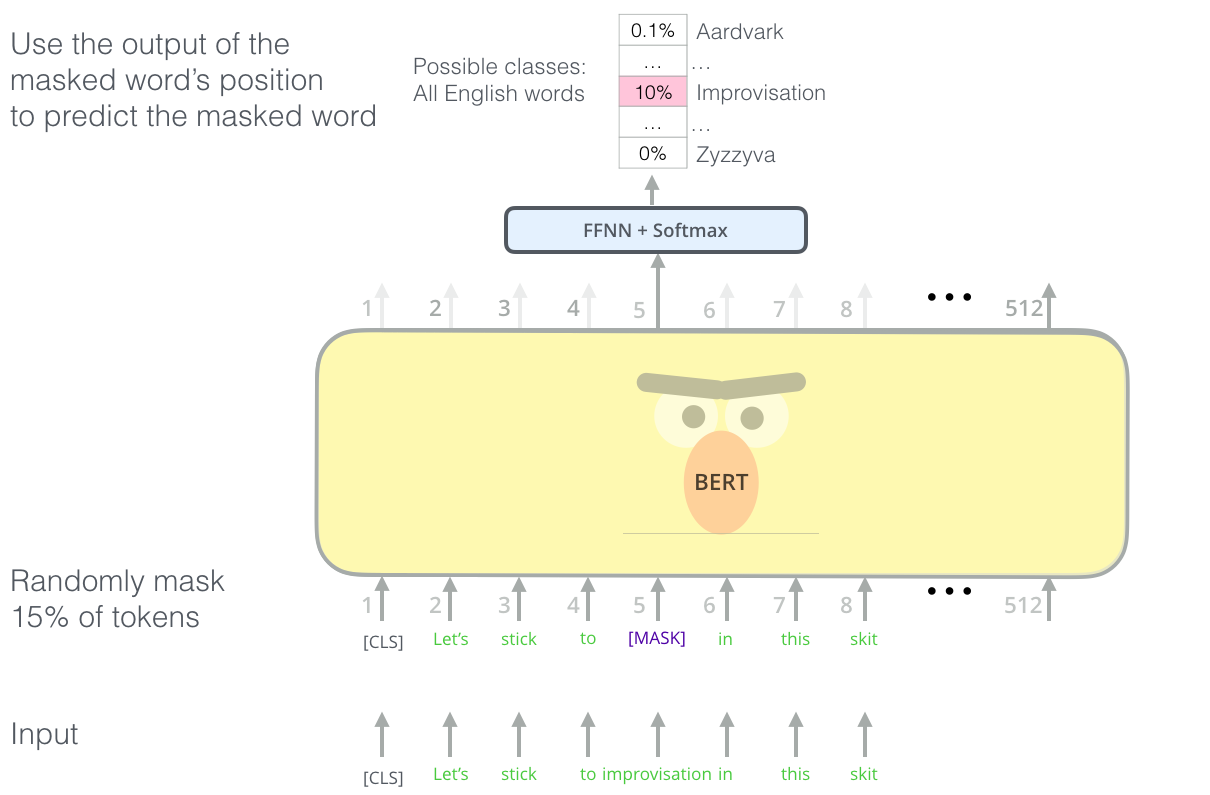
\includegraphics[width=0.9\textwidth]{fig/BERT-language-modeling-masked-lm.png}
\caption{Masked Language Modeling (Alammar, 2019)}
\end{figure}

\end{frame}


\begin{frame}{Next Sentence Prediction}

\begin{figure}[h]
\centering
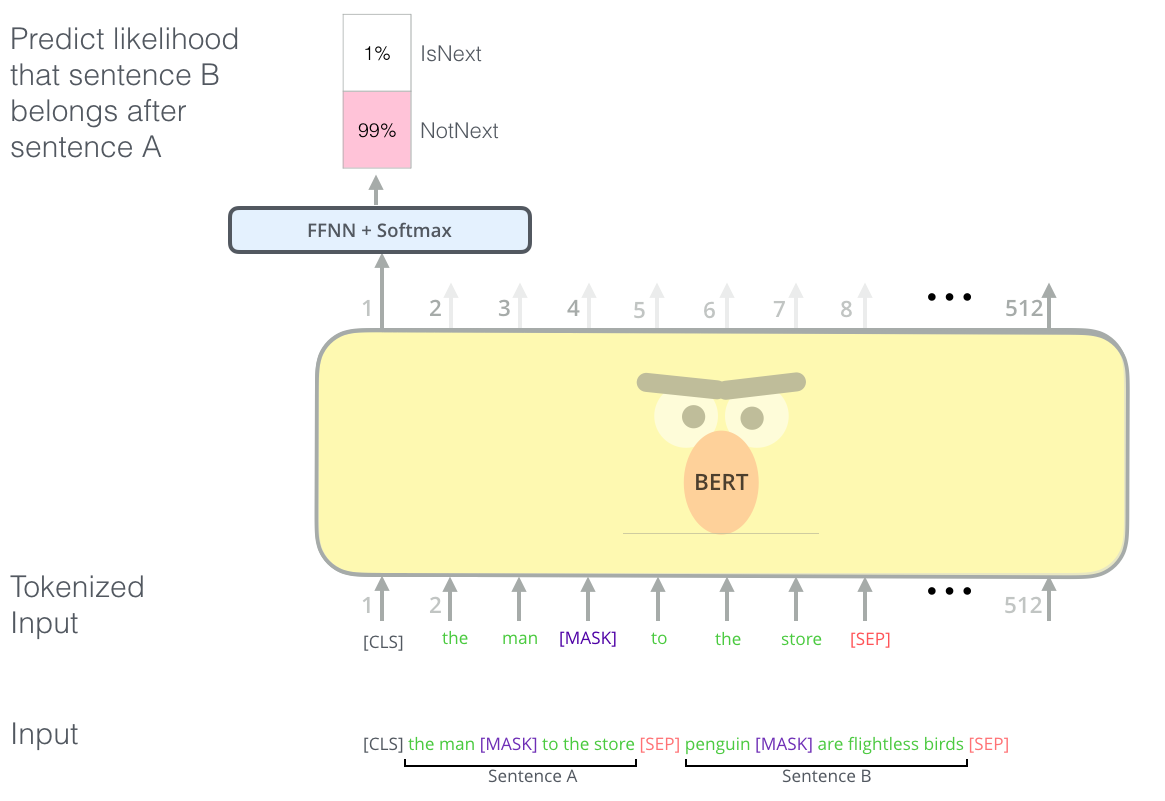
\includegraphics[width=0.9\textwidth]{fig/bert-next-sentence-prediction.png}
\caption{Next Sentence Prediction (Alammar, 2019)}
\end{figure}

\end{frame}



\subsection{Using BERT}

\begin{frame}{Using BERT for Classification}

\begin{figure}[h]
\centering
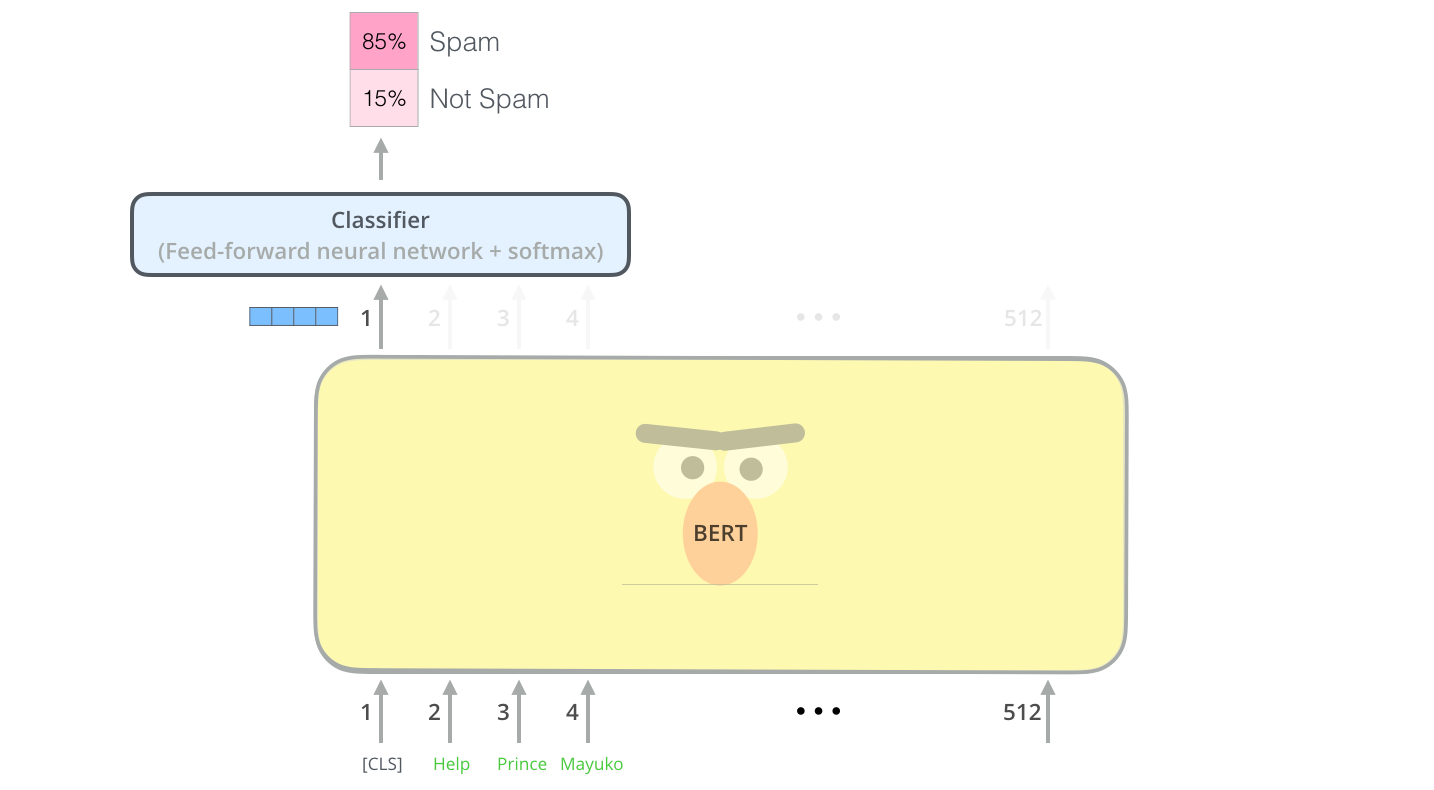
\includegraphics[width=0.9\textwidth]{fig/bert-classifier.png}
\caption{Using BERT for classification (Alammar, 2019)}
\end{figure}

\end{frame}

\begin{frame}{BERT and Contextualized embeddings}

\begin{figure}[h]
\centering
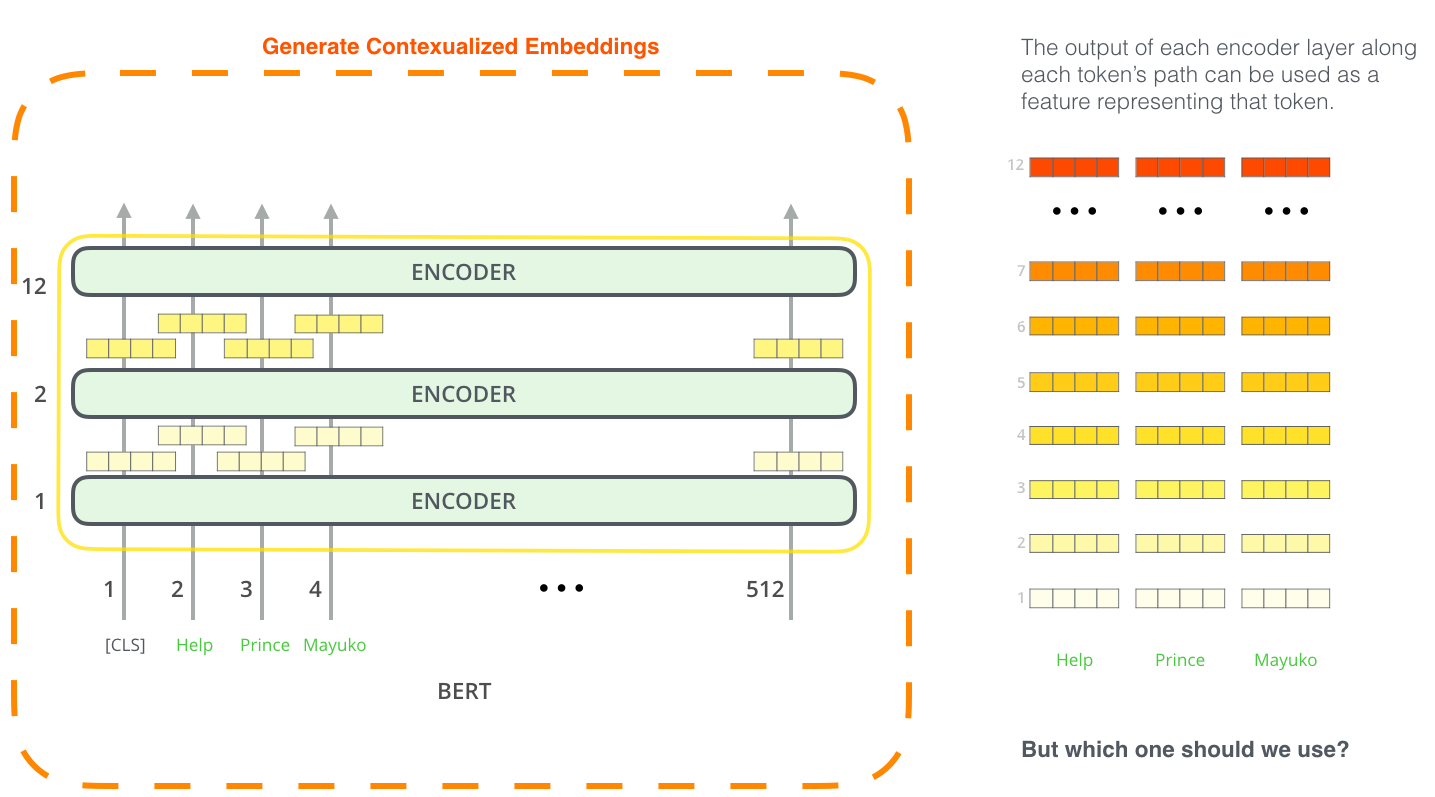
\includegraphics[width=0.9\textwidth]{fig/bert-contexualized-embeddings.png}
\caption{Contextualized Embeddings (Alammar, 2019)}
\end{figure}

\end{frame}

\begin{frame}{Using Contextualized Embeddings}

\begin{figure}[h]
\centering
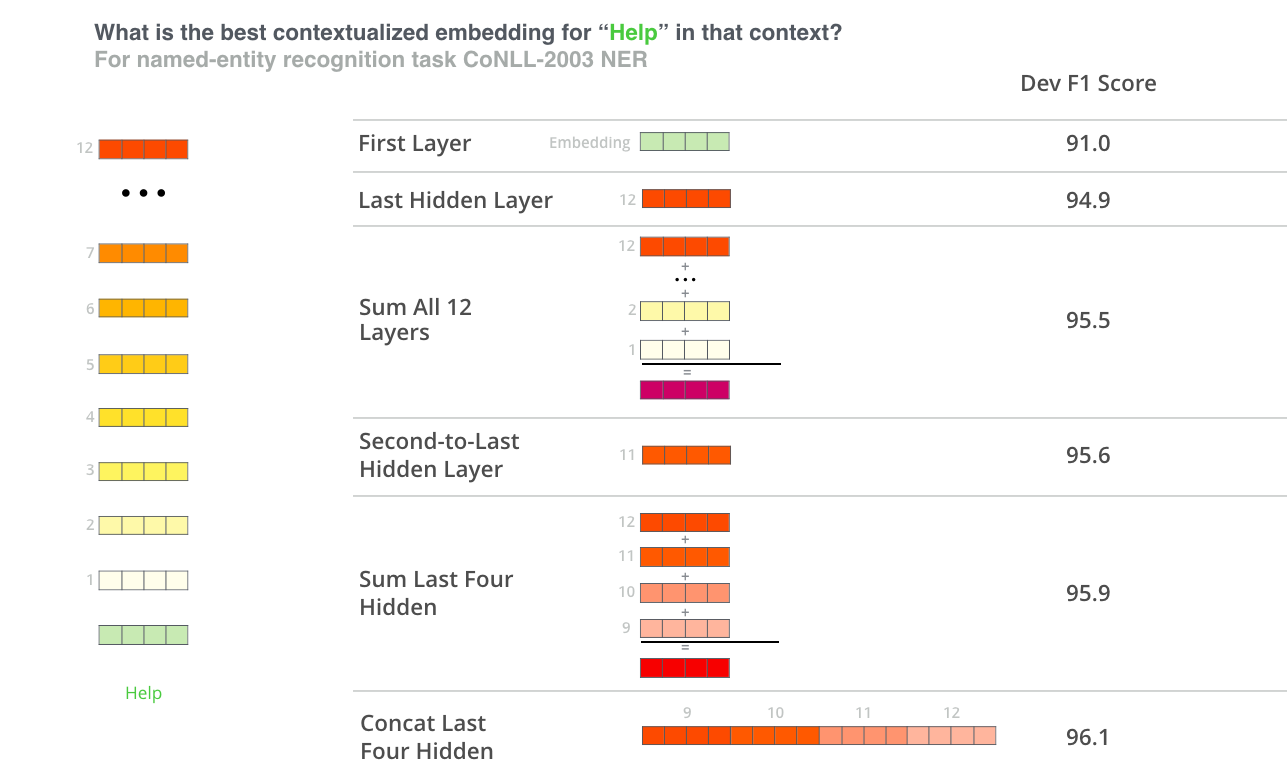
\includegraphics[width=0.9\textwidth]{fig/bert-feature-extraction-contextualized-embeddings.png}
\caption{Using Contextualized Embeddings (Alammar, 2019)}
\end{figure}

\end{frame}




\end{document}
